\documentclass[a4paper,12pt]{monografia}
\usepackage{amsmath,amsthm,amsfonts,amssymb}
\usepackage{latexsym}
\usepackage[brazil]{babel}
\usepackage[utf8]{inputenc}
\usepackage{graphicx}
\usepackage{hyperref}
\usepackage[none]{hyphenat}
\usepackage[alf]{abntex2cite}
\usepackage{graphicx}	
\usepackage{float}
\usepackage{xcolor,colortbl}
\usepackage{longtable}
\usepackage{caption}
\usepackage{fancyhdr}
\pagestyle{fancyplain}
\fancyhf{}
\renewcommand{\headrulewidth}{0pt} % remove lines as well
\rhead{ \fancyplain{}{\thepage} }
\renewcommand{\rmdefault}{phv} % Arial
\renewcommand{\sfdefault}{phv} % Arial

\captionsetup{%
figurewithin=none,
tablewithin=none,  
}
\addto\captionsbrazil{
\renewcommand{\tablename}{Quadro}
}
\tolerance=1
\emergencystretch=\maxdimen
\newcommand{\mc}[2]{\multicolumn{#1}{c}{#2}}
\definecolor{Gray}{gray}{0.85}
\definecolor{ballblue}{rgb}{0.13, 0.67, 0.8}
\newcolumntype{a}{>{\columncolor{Gray}}l}
\newcolumntype{b}{>{\columncolor{white}}c}
\begin{document}
%
%----------------- Título e Dados do Autor -----------------
\titulo{Sudo Loja: Sistema de Gerenciamento de Conteúdo Voltado ao E-Commerce}
\autor{João Marcos Ferreira} \nome{João Marcos} \ultimonome{Ferreira}
%
%---------- Informe o Curso e Grau -----
\tecnologo \curso{Análise e Desenvolvimento de Sistemas} \ano{2016}
\data{dd/MM/2016} % data da aprovação
\cidade{Cajazeiras/PB}
%
%----------Informações sobre a Instituição -----------------
\instituicao{Instituto Federal de Educação Ciência e Tecnologia da Paraíba} \sigla{IFPB}
\unidadeacademica{}
%
%-------- Informações obtidas na Biblioteca ----------------
%
% \CDU{123.45} \areas{Areas..}

\npaginas{55}  % total de páginas do trabalho
%------Nomes do Orientador, 1o. Examinador e 2o.
\orientador{Francisco Paulo de Freitas Neto}
\abrevttorientador{Prof. Msc}
\examinadorum{Examinador 1}
\examinadordois{Examinador 2}
\ttorientador{Orientador}
\ttexaminadorum{Examinador}
\ttexaminadordois{Examinador}
\maketitle
%----------------------------dedicatória--------------
\begin{dedicatoria}
Aos meus pais e irmãos.\\
Aos meus amigos\\
\end{dedicatoria}

%----------------------------Agradecimentos--------------
\agradecimento{Agradecimentos}
\noindent Primeiramente a Deus. O que seria de nós sem Ele?	\\
Aos meus pais que sempre me incentivaram e ajudaram, sem eles não teria chegado até aqui.\\
Ao meu Orientador Francisco Paulo de Freitas Neto pela paciência, disponibilidade e por prestar toda a orientação e esclarecimentos necessários.\\
Aos meus tios Isabel e Alonso por me acolherem durante todos esses dias.\\
À minha namorada por estar sempre ao meu lado me encorajando\\
Aos meus amigos e todos os meus parentes pelo apoio.

\newpage

%--------Resumo em Português--------------
\resumo{Resumo} 

Na atualidade muitas pessoas preferem fazer suas compras em casa usando seu computador ou \textit{smartphone}, ao invés de se deslocarem até uma loja ou supermercado. Com um número de pedidos no \textit{e-commerce} aumentando cada vez mais e movimentando quantias cada vez maiores, percebe-se que é um mercado em ascensão. Os comerciantes da região ainda desconhecem ferramentas que facilitam a criação e gestão de uma loja virtual. Este trabalho apresenta uma ferramenta capaz de criar, gerenciar e personalizar uma loja virtual. O uso desta ferramenta trará benefícios a aqueles interessados em vender na Internet, pois poderão com facilidade, sem burocracias, sem custos elevados, e sem precisar ter conhecimentos avançados sobre programação, criar e gerir seu próprio \textit{e-commerce}.

\noindent \textbf{Palavras-chaves:} Sistemas de Gerenciamento de Conteúdo. Loja Virtual. Vendas.
%-----------Resumo em Inglês--------------
\resumo{Abstract} 

Nowadays many people prefer to do their shopping at home using your computer or smartphone, instead of moving to a store or supermarket. With a number of requests in e-commerce continually increasing and moving increasingly larger amounts, it is clear that it is a growing market. Traders in the region are still unaware of tools that facilitate the creation and management of a virtual store. This paper presents a tool to create, manage and customize a virtual store. Use of this tool will benefit those interested in selling on the Internet, they may easily, without bureaucracy, without high costs and without having advanced knowledge about programming, create and manage your own e-commerce.

\noindent \textbf{Keywords:} Content Management System. Virtual Store. Sales.
\newpage

%---------------------- EPÍGRAFE I (OPCIONAL)--------------
\begin{epigrafe}
“Pequenas oportunidades são muitas vezes o começo de grandes empreendimentos.”\\
\hfill Demóstenes
\end{epigrafe}

%----Sumário, lista de figuras, quadros------------
\addtocontents{toc}{\protect\setcounter{tocdepth}{-1}}

{% Lista de Figuras 
\let\oldnumberline\numberline%
\renewcommand{\numberline}{\figurename~\oldnumberline}%
\listoffigures%
\thispagestyle{empty}
}

\renewcommand\listtablename{Lista de Quadros}

{% Lista de Quadros
\let\oldnumberline\numberline%
\renewcommand{\numberline}{\tablename~\oldnumberline}%
\listoftables%
\thispagestyle{empty}
}

\addtocontents{toc}{\protect\setcounter{tocdepth}{2}}
\tableofcontents
\thispagestyle{empty}
%---------------------
% 
\chapter{Introdução} % (fold)
\label{cha:intro}

Comprar na Internet traz muitas vantagens para um consumidor. É possível fazer compras sempre que quiser e à hora que desejar, no conforto da sua casa; Não existem filas; As compras são feitas sem a utilização de dinheiro físico, proporcionando mais segurança ao cliente, além de diversas outras vantagens.

Para os comerciantes as vantagens também são muitas: o produto fica acessível aos clientes 24 horas por dia, todos os dias da semana; pessoas de todos os lugares podem ver o produto; não é necessário um espaço físico para expor os produtos; custo de investimento inicial mínimo; sem risco de assalto, entre outras.

Dados indicam que os consumidores virtuais demonstram altos índices de intenção de compra, ou seja, continuam consumindo apesar do estabelecimento de um cenário de crise, e principalmente na Internet, onde os preços geralmente são mais baratos, se comparados aos do varejo tradicional \cite{webshoppers}.

O \textit{WebShoppers} \citeonline{webshoppers}, relatório sólido e respeitado sobre o comércio eletrônico anualmente publicado, no qual são analisadas a evolução do \textit{e-commerce}, tendências, estimativas, mudanças de comportamento e preferências dos e-consumidores, apresentou boas estatísticas sobre o \textit{e-commerce} no Brasil. A seguir serão apresentados dados em forma de figuras e gráficos.

A figura \ref{figura:consumidores} apresenta a quantidade de e-consumidores ativos (pessoas que efetivaram pelo
menos uma compra virtual, ao longo de 2015). Percebe-se um crescimento, se comparada com anos anteriores. Em 2015, esse número chegou ao total de 39,1 milhões de consumidores.

\begin{figure}[H]
\centering
\caption{Consumidores únicos ativos}
\centering
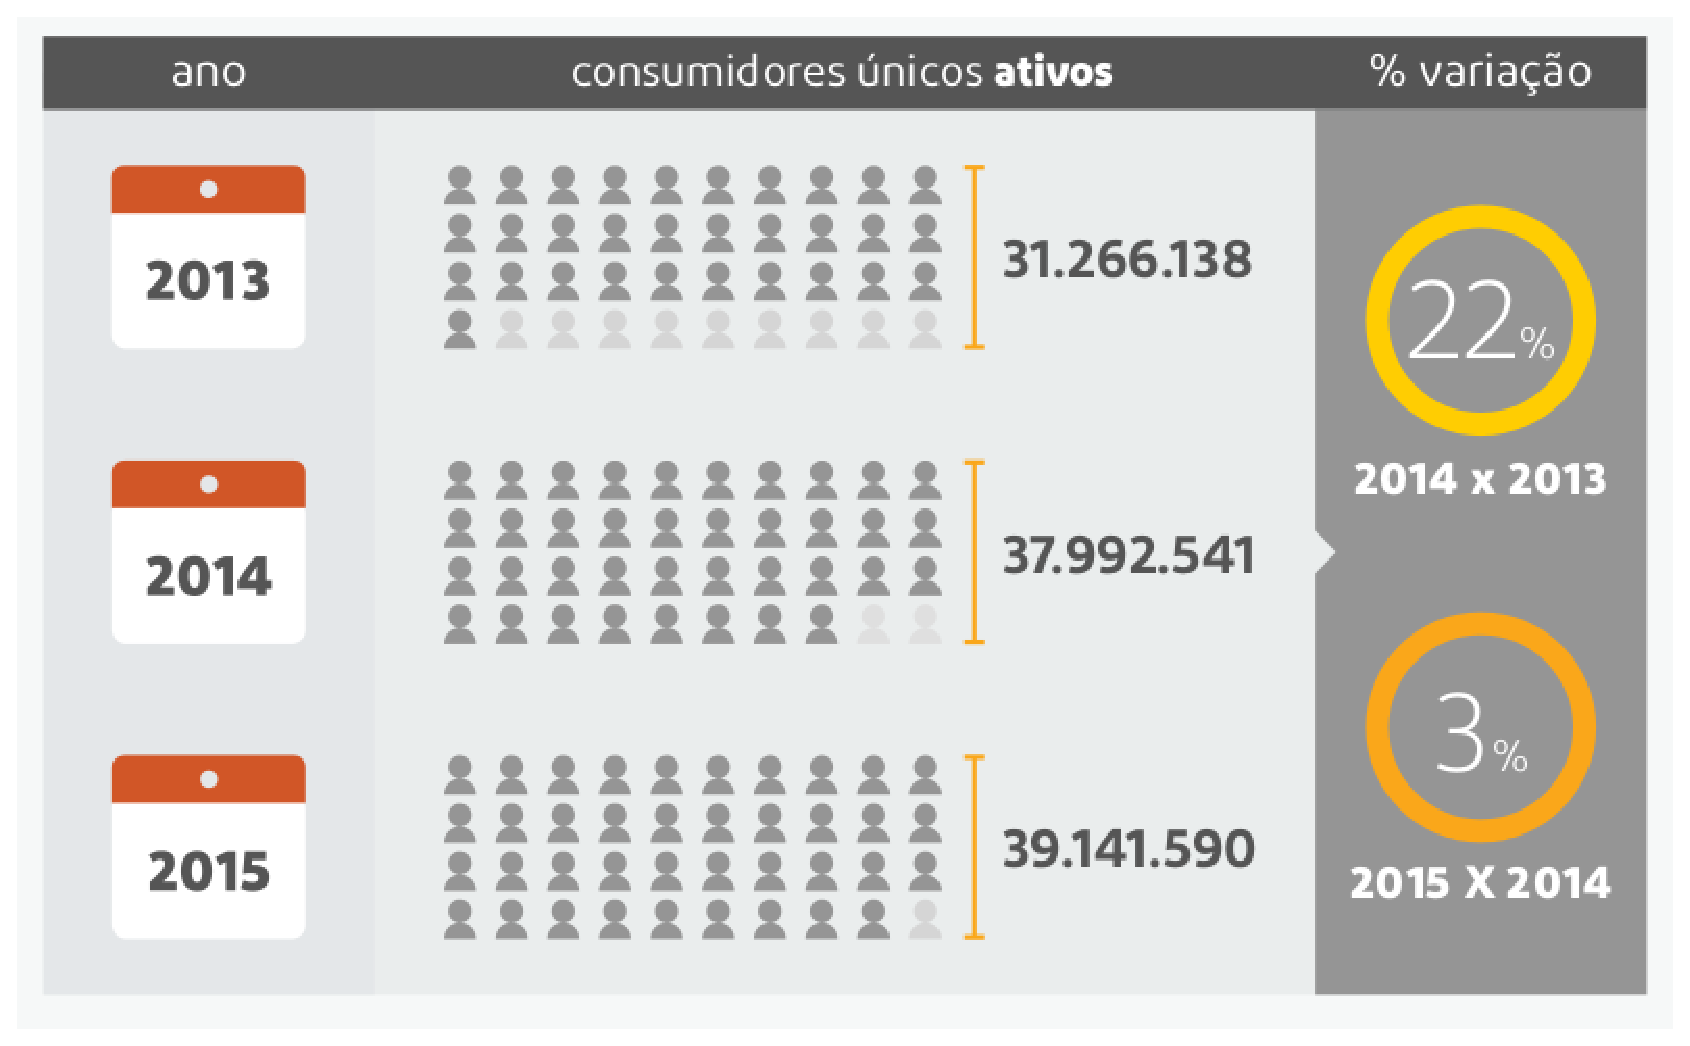
\includegraphics[width=12cm]{img/webshoppers/consumidores.eps}\\
\small{Fonte: \citeonline{webshoppers} - Relatório WebShoppers}
\label{figura:consumidores}
\end{figure}

O número de pedidos e o faturamento do comércio eletrônico também foram notavelmente altos. Como mostra a figura \ref{figura:pedidos}, com um total de 106,2 milhões em 2015, o incremento no número de pedidos no mercado brasileiro foi de 3\%, em relação a 2014. O faturamento do comércio eletrônico foi de R\$ 41,3 bilhões. O número representa um crescimento nominal de 15,3\%, em relação a 2014, quando as vendas somaram um total de R\$ 35,8 bilhões como pode ser visto na figura \ref{figura:vendas}.

\begin{figure}[H]
\centering
\caption{Total de pedidos realizados no \textit{e-commerce} no Brasil}
\centering
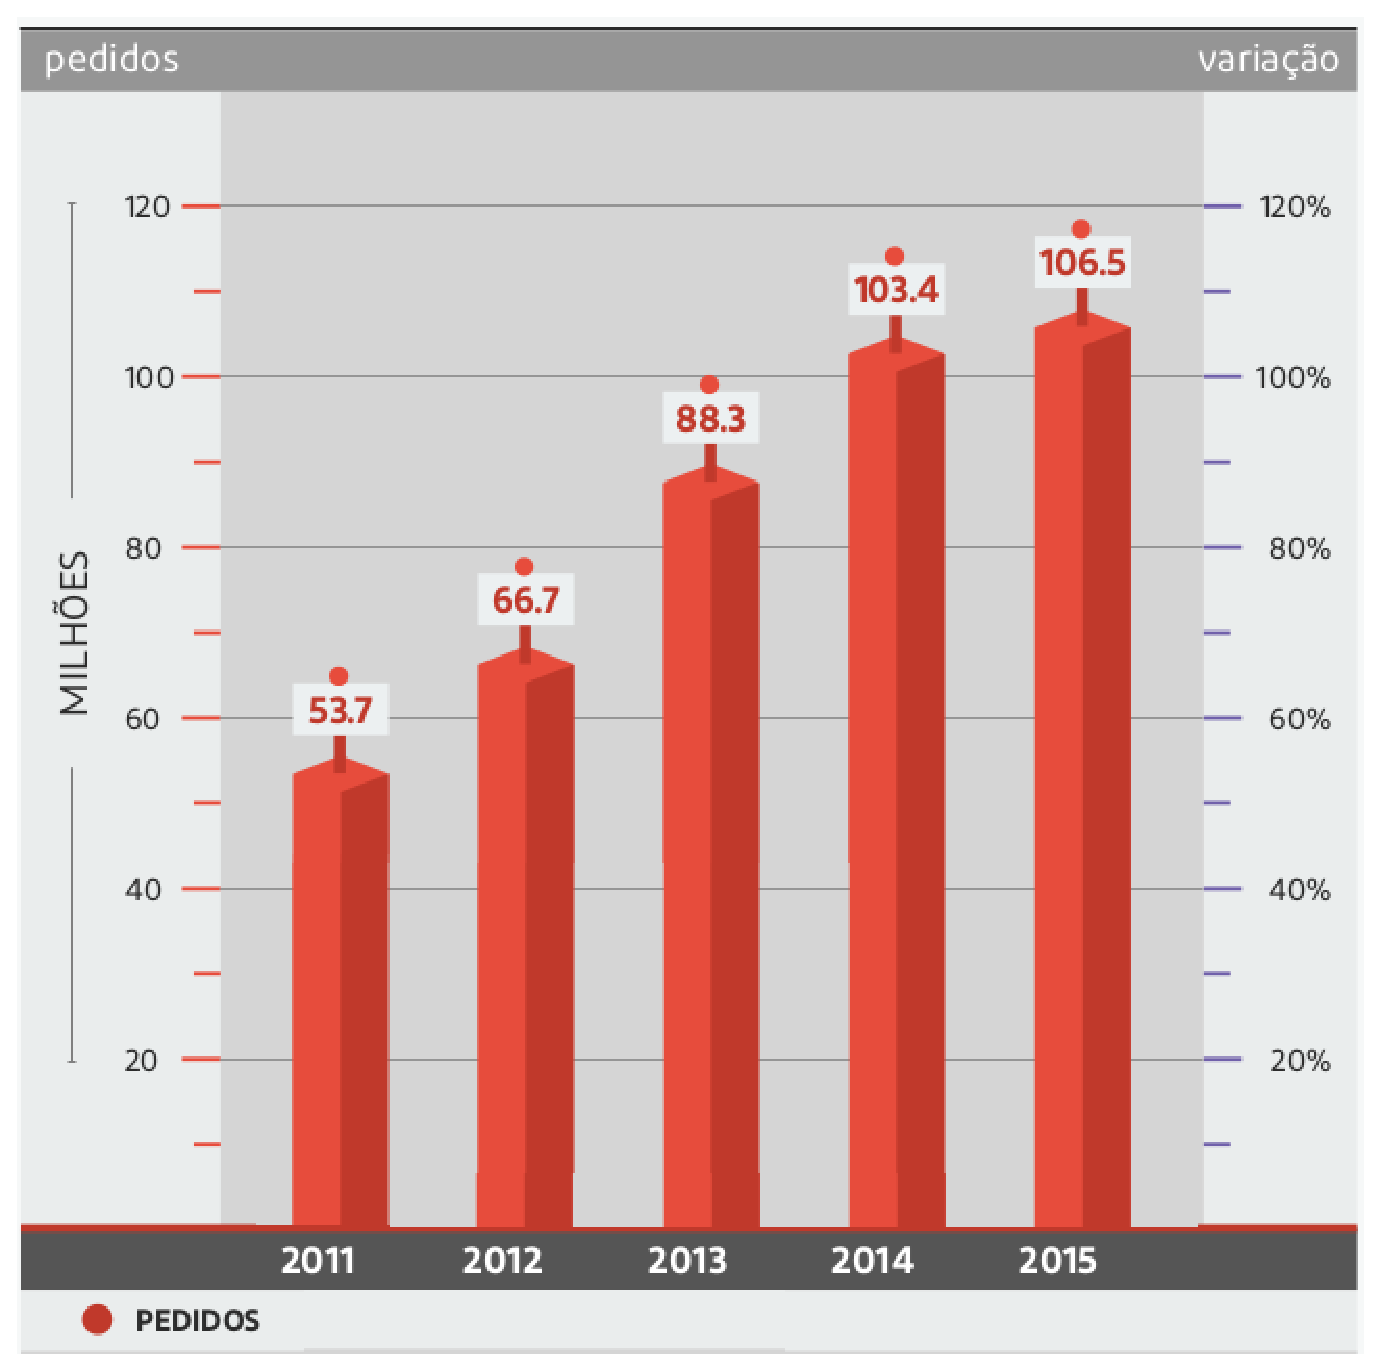
\includegraphics[width=10cm]{img/webshoppers/total-pedidos.eps}\\
\small{Fonte: \citeonline{webshoppers} - Relatório WebShoppers}
\label{figura:pedidos}
\end{figure}

\begin{figure}[H]
\centering
\caption{Total de faturamento do \textit{e-commerce} no Brasil}
\centering
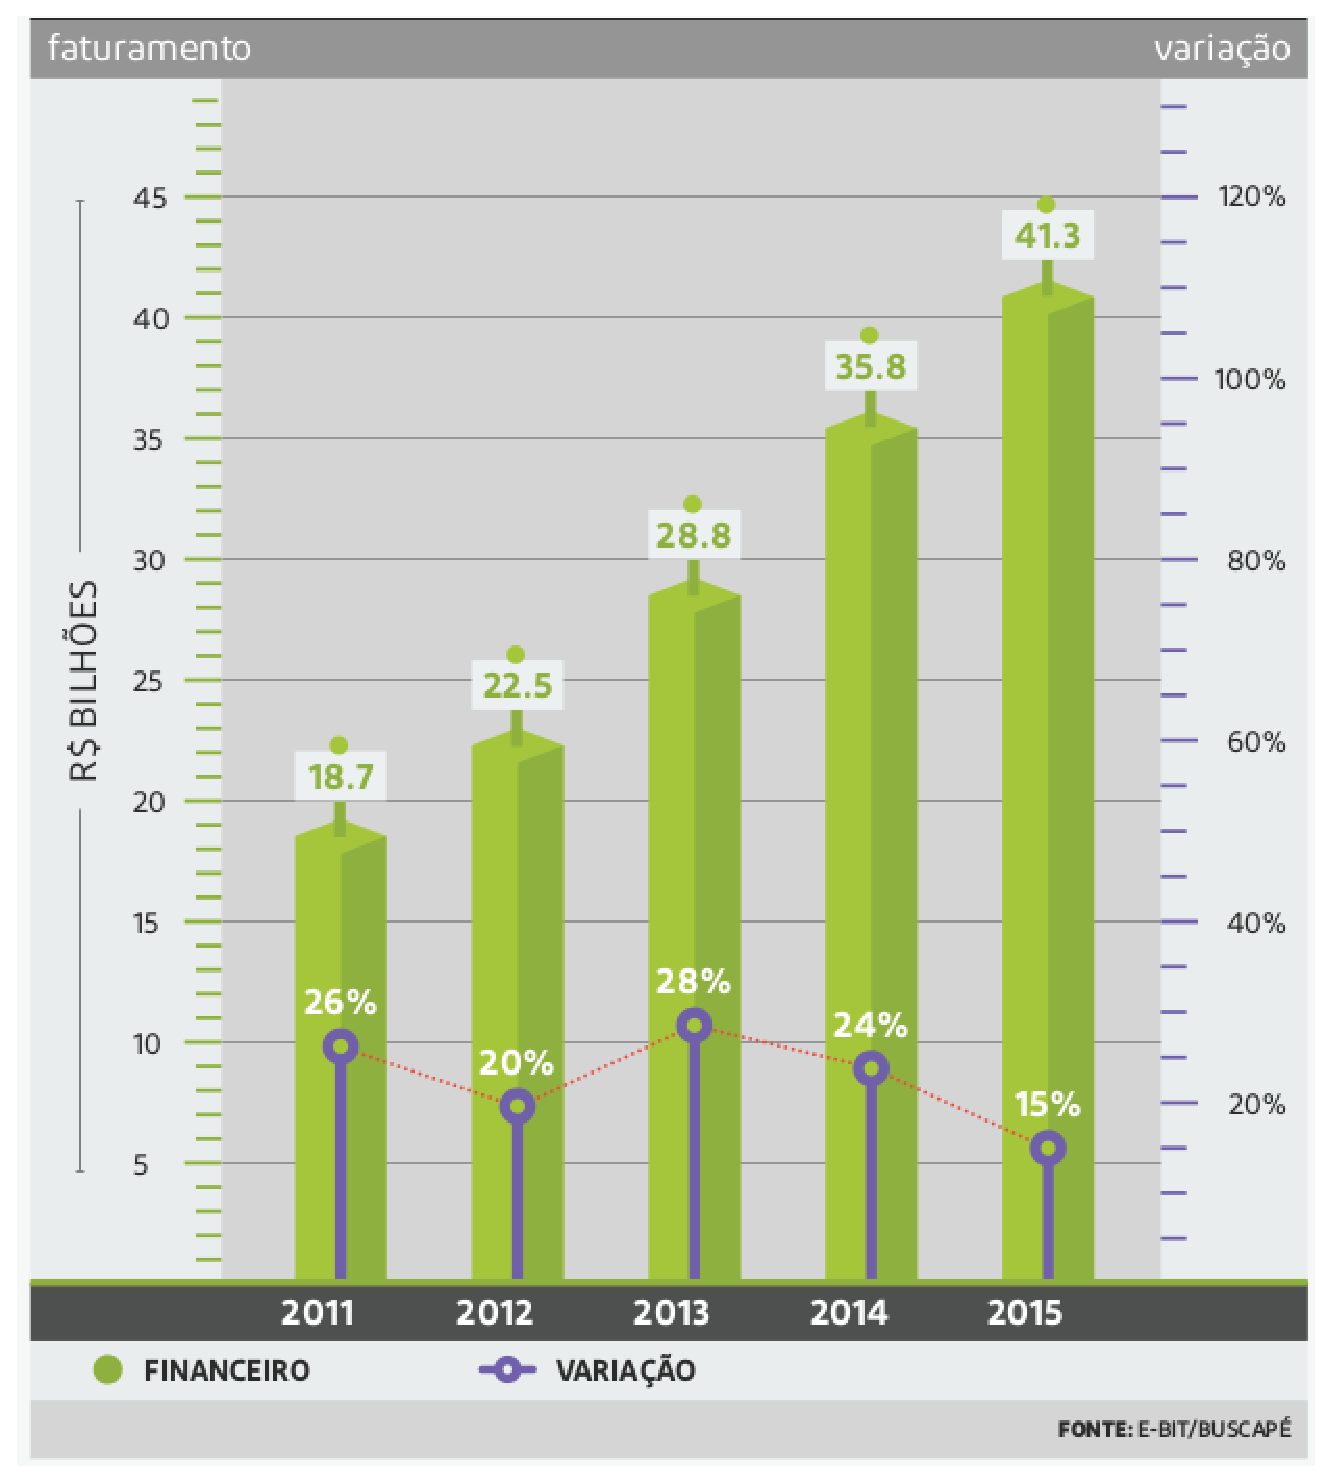
\includegraphics[width=10cm]{img/webshoppers/faturamento.eps}\\
\small{Fonte: \citeonline{webshoppers} - Relatório WebShoppers}
\label{figura:vendas}
\end{figure}

O relatório também destaca dados sobre a satisfação dos clientes em realizar suas compras na internet. O Net Promoter Score (NPS) é um indicador que mensura a satisfação e a fidelização dos clientes. No balanço geral do ano, o NPS apresentou o melhor resultado. A figura \ref{figura:nps} apresenta esse dados.

\begin{figure}[H]
\centering
\caption{Satisfação e fidelização de clientes}
\centering
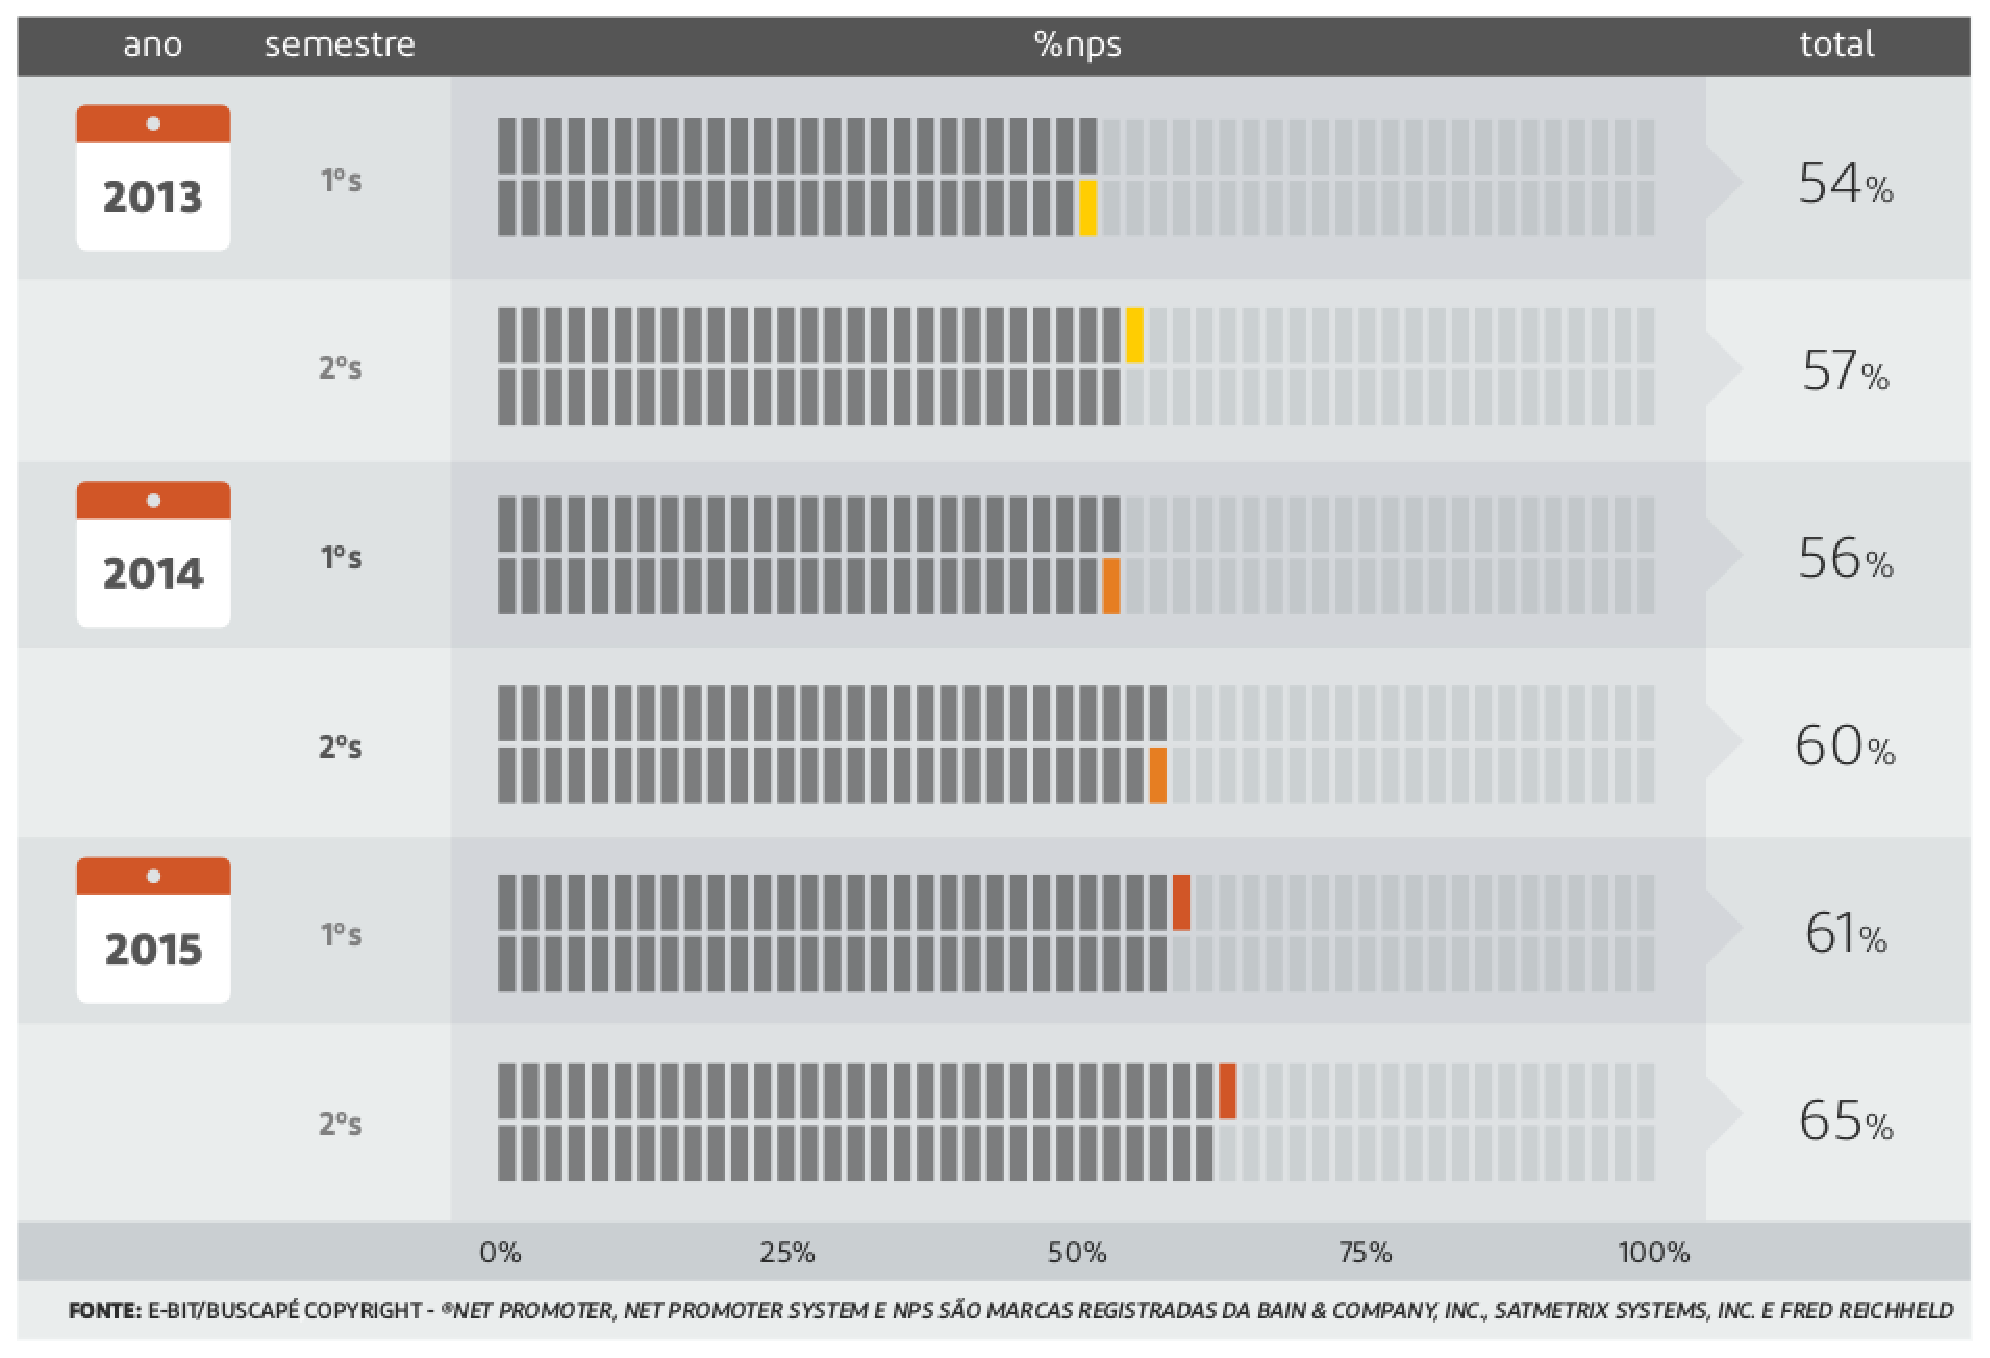
\includegraphics[width=12cm]{img/webshoppers/nps.eps}\\
\small{Fonte: \citeonline{webshoppers} - Relatório WebShoppers}
\label{figura:nps}
\end{figure}

Vitor Augusto Meira França, economista da Fecomercio-SP principal entidade sindical paulista dos setores de comércio e serviços. Responsável por administrar, no Estado, o Serviço Social do Comércio (Sesc) e o Serviço Nacional de Aprendizagem Comercial (Senac) afirma o seguinte:

\begin{citacao}
Diante de um quadro de instabilidade política, inflação alta, taxas de juros elevadas, escassez de crédito, aumento do desemprego e consequente conservadorismo dos consumidores, o varejo brasileiro deve repetir o fraco desempenho do ano passado e registrar nova queda das vendas neste ano. por outro lado, o e-commerce deve apresentar crescimento como ocorreu em 2015. \cite{webshoppers}
\end{citacao}

A figura \ref{figura:estimativa:faturamento} apresenta estimativas relacionadas ao faturamento do \textif{e-commerce}, para o ano de 2016, no Brasil.

\begin{figure}[H]
\centering
\caption{Estimativa de faturamento do \textit{e-commerce} para 2016}
\centering
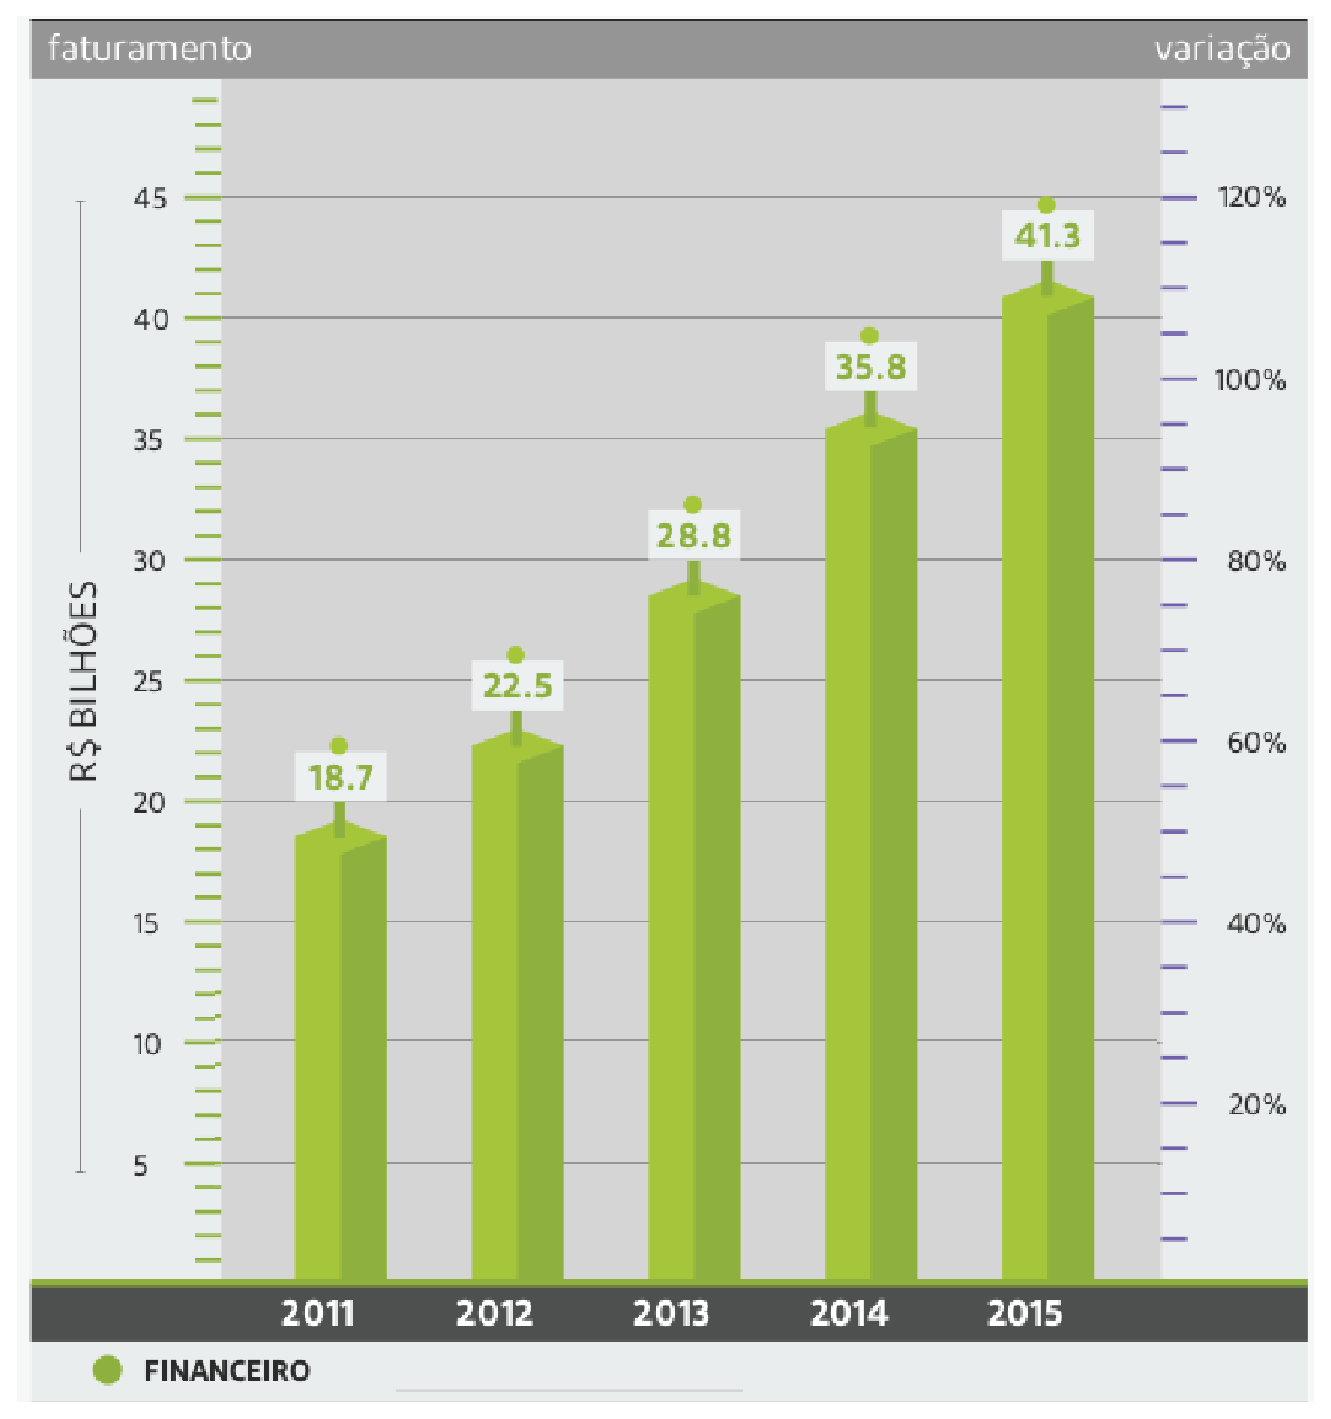
\includegraphics[width=12cm]{img/webshoppers/estimativa-faturamento.eps}\\
\small{Fonte: \citeonline{webshoppers} - Relatório WebShoppers}
\label{figura:estimativa:faturamento}
\end{figure}

Diante esses dados sobre o \textit{e-commerce} no brasil, percebe-se que o comércio eletrônico é um mercado em ascensão.

Entre os empresários que se aventuram nesse ambiente, um dos anseios é ter uma loja que tenha a identidade visual da sua marca, que possibilite formas práticas e seguras de compra pelos clientes e, claro, que seja de fácil manuseio e administração para ele mesmo. Com ferramentas como o Mercado Livre\footnote{https//www.mercadolivre.com.br}, por exemplo, é possível disponibilizar produtos para a venda, mas em um ambiente diferente de uma loja virtual particular.
% chapter introdução(end)

\section{Motivação} % (fold)
\label{sec:motivacao}

Existem muitas ferramentas que facilitam a criação e gestão de lojas virtuais, porém algumas delas não são populares e as vezes desconhecidas, tais ferramentas poderiam ajudar a expandir um negócio ou criar uma oportunidade para aqueles que desejam empreender através de vendas na Internet. 

Segundo \citeonline{felipini}, \textit{Um e-commerce pode ser implantado aos poucos e testado}. Diferentemente de uma empresa tradicional, em que o início das operações ocorre somente com o empreendimento totalmente estruturado, um negócio na Internet pode ser implantado em etapas, o que dilui o investimento e facilita a correção de erros. Por exemplo, um estabelecimento de vendas só receberá seu primeiro cliente após a loja estiver totalmente pronta. Na Internet, você pode montar um site de conteúdo, com ou sem sua marca definitiva, testar a aceitabilidade de seu modelo de negócio e produtos, avaliar a visitação e, somente depois, começar a vender. Dessa forma, mesmo aqueles que ainda não possuam um negócio, poderão investir em um \textit{e-commerce}.

Os comerciantes já fixados no mercado e interessados em colocar seu negócio na rede, procuram por empresas especializadas em desenvolvimento de softwares para desenvolver seu site de vendas. O problema nisso é que o custo pode ser alto. \citeonline{jalote} afirma: \textit{O software é caro porque torna se uma atividade difícil e trabalhosa de ser realizado pelo engenheiro de software}.  Outro problema relacionado ao desenvolvimento de software no geral, isso inclui uma loja virtual, é o tempo. O que gera insatisfação dos clientes, pela demora no cumprimento dos prazos \cite{pressman}.

Além desses, um outro problema é a manutenção do site. Segundo \citeonline{sommervile} manutenção de software é a modificação de um programa após ter sido colocado em uso. Mudanças por exemplo, em alterar o \textit{layout}\footnote{Aspecto visual das páginas do site} geram custos e podem também ser demoradas.

A Sudo Loja, visa resolver esses problemas oferecendo um CMS (do inglês \textit{Content Management System}), capaz de criar, gerenciar e tornar possível a personalização de uma loja virtual. O CMS proposto busca facilitar a criação e gestão de um \textit{e-commerce}, promovendo uma entrada rápida ao mercado virtual à pequenas e médias empresas. Podem ser vistos vários sistemas que funcionam dessa maneira, como por exemplo: a Tray commerce\footnote{https://www.tray.com.br/} e Loja integrada\footnote{https://lojaintegrada.com.br/}. Na Seção \ref{sec:ferramentas_relacionadas} será apresentado um comparativo entre estas e outras ferramentas.


% section motivacao (end)

\section{Objetivos} % (fold)
\label{sec:objetivos}

Esta seção apresenta os objetivos que direcionarão a construção do sistema.

\subsection{Objetivo Geral} % (fold)
\label{sub:objetivo_geral}

Esse trabalho tem como objetivo principal o desenvolvimento de uma ferramenta para criação de lojas virtuais, onde um usuário cadastrado poderá criar um ou mais lojas, personalizar seu \textit{layout} e disponibilizar produtos para a venda.

% subsection objetivo_geral (end)

\subsection{Objetivos Específicos} % (fold)
\label{sub:objetivos_espec}

\begin{itemize}
\item Prover uma alternativa de \textit{e-commerce} para a região.
\item Incentivar o uso de novas soluções em TI nas pequenas e médias empresas comerciais da região.
\item Facilitar a entrada de novos comerciantes no mercado virtual.
\item Desenvolver um painel administrativo para que os usuários possam acompanhar e gerenciar sua loja.
\item Tornar possível a criação de mais de uma loja com a mesma conta de usuário.
\item Disponibilizar um módulo para personalização das lojas.
\end{itemize}
% subsection objetivos_espec (end)

% section objetivos (end)

\section{Organização do Documento} % (fold)
\label{sec:organizacao_do_documento}

% section organizacao_do_documento (end)
A Seção \ref{cha:fundamentaco_teorica} apresenta a fundamentação teórica para o desenvolvimento deste trabalho. Na Seção \ref{cha:metodologia} é descrita a metodologia adotada para execução do projeto. A Seção \ref{cha:sudoloja} descreve a solução proposta no trabalho, um comparativo entre ferramentas do gênero e também as etapas de análise, projeto, implementação e validação do sistema. A Seção \ref{cha:considera_es_finais} apresenta as considerações finais do trabalho, assim como discussões sobre trabalhos futuros. Por fim, os artefatos gerados no decorrer do desenvolvimento do trabalho podem ser vistos nos Apêndices.

\chapter{Fundamentação Teórica} % (fold)
\label{cha:fundamentaco_teorica}

Essa seção discutirá sobre alguns assuntos necessários para obter um melhor entendimento do trabalho.

\section{CMS} % (fold)
\label{sec:cms}

Sistemas de Gerenciamento de Conteúdo (SGC) ou Content Management System (CMS), segundo \citeonline{mercer} são softwares que facilitam a criação, organização, manipulação e remoção de dados em forma de imagens, documentos, scripts, textos, etc.
Já \citeonline{barcia}, diz que um CMS, é uma plataforma de gestão de conteúdos, ou seja, um sistema que integra ferramentas que permitem criar, editar e publicar conteúdo em tempo real, onde os utilizadores manipulam uma interface sem terem a necessidade de saber programar. \citeonline{barcia} ainda ressalta que os gerenciadores também dispensam o uso de programação, facilitando dessa forma a gestão dos dados e o acesso às funcionalidades da ferramenta.

O uso de um CMS pode facilitar o trabalho dos administradores de aplicações, que envolvem muitas atualizações no seu conteúdo, como por exemplo, blogs, portais corporativos\footnote{Instrumento de gestão de informação e de conhecimento}. \textit{Os benefícios ligados a adoção de um CMS incluem desde a redução do custo de atualização dos conteúdos nos web sites até o aumento da eficiência das equipes de TI} \cite{pereira}.

Em linhas gerais, um CMS permitiria administrar conteúdos em meio digital. E para o caso particular desse trabalho, um CMS permitiria gerenciar os conteúdos de uma loja virtual.

Em outras palavras, um CMS é uma ferramenta que permite a um editor criar e publicar qualquer tipo de informação em uma página web. Geralmente, um CMS trabalha manipulando um banco de dados, de modo que o editor simplesmente atualiza este banco, incluindo nova informação ou editando a existente.

Contudo, o mais interessante, é que essa ferramenta é feita de tal maneira que mesmo aqueles que nunca ouviram falar de JAVA, PHP, MySQL, Javascript ou qualquer outra linguagem voltada para web poderá utilizá-la, inclusive esta é sua principal função, tornar acessível a todos a sua presença na Internet através de um site, facilitando a inserção de textos, de comentários e dezenas de outras funcionalidades, de acordo com as características de cada aplicação. Alguns Exemplos de CMS podem ser vistos a seguir.

\begin{itemize}
\item \textit{Drupal} - É uma plataforma de gerenciamento de conteúdo de código aberto, usado em milhares de web sites e aplicações. Ele é desenvolvido, usado, e apoiado por uma comunidade ativa e diversificada de pessoas ao redor do mundo \cite{drupal}.

\item \textit{OpenText} \citeyear{opentext} - O primeiro sistema CMS comercial que apareceu no mercado. A OpenText é líder em Gestão de Informação Corporativa. Seus produtos de gerenciamento de conteúdo permitem uma coleta mais eficiente de todos os tipos de informação - estruturada e não estruturada - e fornecem essa informação em contexto por qualquer aplicativo, plataforma ou processo \cite{opentext}.

\item \textit{Wordpress} - Sistema muito popular e bastante usado pelos \textit{bloggers}. WordPress é um software web que você pode usar para criar um site, blog, ou app \cite{wordpress}.
\end{itemize}

% section cms (end)

\section{\textit{E-commerce}} % (fold)
\label{sec:e_commerce} 

Segundo \citeonline{kalakota}, o Comércio Eletrônico (CE) pode ser definido como sendo a compra e a venda de informações, produtos e serviços através de redes de computadores. \citeonline{bloch} estenderam esta definição incluindo que CE (Comércio Eletrônico) é o suporte para qualquer tipo de transações de negócio sobre uma infraestrutura digital.

\apudonline{kalakota}{albertin} há muito tempo, consideravam que o ambiente tradicional de negócio estava mudando rapidamente, com os consumidores e negócios procurando flexibilidade para mudar os parceiros de negócio, plataformas, carreiras e redes. O \textit{e-commerce} começava a se disseminar.

\begin{citacao}
	O comércio eletrônico ou \textit{e-commerce}, é aplicável a qualquer tipo de transação comercial que pode envolver compra, venda, transferência ou troca de produtos, serviços ou informações por meio de redes de computadores, incluindo a Internet \cite{turban}.
\end{citacao}

Existem diferenças entre \textit{e-commerce} e \textit{e-business}. \textit{E-business} é definido como o uso das tecnologias da informação para executar funções de negócios. \textit{E-business} é, portanto, um termo mais amplo que inclui \textit{e-commerce} \cite{gordon}. 

Dentre os modelos existentes de \textit{e-business}, \citeonline{asfoura} destacam três tipos principais que incluem o e-commerce em sua execução:

\begin{itemize}
\item \textbf{Empresa para Empresa (B2B – Business to Business):} Engloba as negociações de bens ou serviços que acontecem entre empresas;
\item \textbf{Empresa para Consumidor (B2C – Business to Consumer):} Tipo de comércio mais conhecido, onde a empresa faz o negócio diretamente com os consumidores finais;
\item \textbf{Consumidor para Consumidor (C2C – Consumer to Consumer):} Engloba todas as transações que acontecem entre consumidores finais, geralmente intermediadas por uma terceira entidade;
\end{itemize}

O sistema que será apresentado se encaixa no modelo de negócio B2C (\textit{Business to Consumer}), onde o lojista fará o negócio diretamente com os consumidores finais.

\section{YP} % (fold)
\label{sec:yp}

Quando se trabalha na elaboração de um produto os sistema, é importante seguir uma série de passos previsíveis - um roteiro que ajude a criar um resultado de alta qualidade e dentro de prazo estabelecido. O roteiro é denominado ``Processo de Software'' \cite{pressman}.

O \textit{easyProcess}, comumente chamado de YP. É um processo de \texit{software} criado com o objetivo de sanar as dificuldades dos alunos em se adaptar aos processos já existentes para o uso na academia. Voltado a projetos de pequeno escopo, o YP foca-se na aprendizagem do processo com alguns elementos qualificadores: uma boa produtividade, bom uso do ferramental de apoio e geração mínima de artefatos, além de se buscar uma consolidação do entendimento das práticas e conceitos da Engenharia de Software \cite{easyprocess}. O fluxo básico do YP está ilustrado na figura \ref{figura:yp}.

\begin{figure}[H]	
\centering
\caption{Fluxo do \textit{easyProcess}}
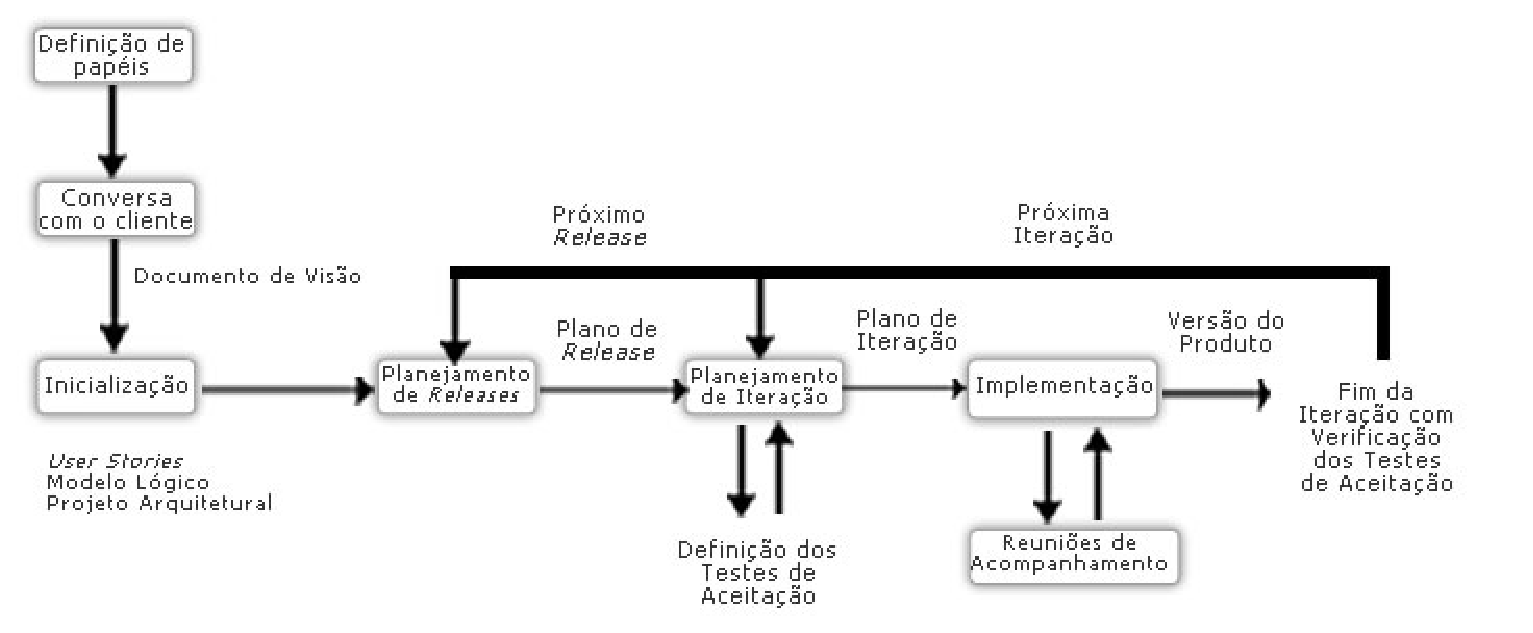
\includegraphics[width=15cm]{img/yp.eps}
\small{Fonte: \cite{easyprocess}}
\label{figura:yp}
\end{figure}

A primeira etapa do processo consiste na \textbf{Definição de papéis}. O YP sugere os seguintes papéis: cliente, usuário, testador, desenvolvedor e gerente, podendo uma mesma pessoa desempenhar mais de um papel dentro do processo, principalmente quando se tratam de equipes de desenvolvimento pequenas \cite{easyprocess}.

Em seguida deve ser realizada uma \textbf{Conversa com o cliente}. Aqui é onde as informações sobre o escopo do problema
são adquiridas. A partir de então, a equipe encontra-se apta a gerar o documento de visão, que após ser validado pelo cliente, funciona como um acordo de trabalho entre cliente e equipe de desenvolvimento \cite{easyprocess}.

Na fase de \textbf{Inicialização} o cliente define as \textit{User Stories}\footnote{Funções que o sistema deve desempenhar e que são definidas pelo cliente e pelo desenvolvedor} e são elaborados o projeto arquitetural e o modelo lógico de dados, este último apenas se necessário. O cliente deve priorizar as User Stories e a equipe deve fazer uma estimativa inicial do tempo para implementação de cada uma delas. Baseado nessa estimativa pode-se então verificar a viabilidade de desenvolvimento do projeto no escopo e tempo definidos \cite{easyprocess}.

Parte-se então para o \textbf{Planejamento} fase composta por dois planos, o de release e o de iteração. Ambos possuem tempo fixo com variação de escopo permitida. Tratando-se do ambiente acadêmico são sugeridos três releases, cada um com duas iterações de duas semanas, por semestre letivo \cite{easyprocess}. 

Para a \textbf{Implementação}, o processo prega o uso de algumas práticas, tais como: \textit{Design} Simples, Padrões de Codificação, Padrões de Projeto, Refatoramento e Propriedade Coletiva de Código, a fim de produzir um código com mais qualidade \cite{easyprocess}. 

O andamento do processo deve ser coordenado pelo gerente através da \textbf{Reunião de Acompanhamento} semanal que visa recolher e analisar métricas.

\section{Bancos de dados NoSQL} % (fold)
\label{sec:bancos_de_dados_nosql}
Os bancos de dados NOSQL surgiram como uma solução para a questão da escalabilidade no armazenamento e processamento de grandes volumes de dados na Web 2.0. No início, grandes empresas enfrentando esse tipo de problema criaram suas próprias soluções e publicaram alguns artigos, mas sem usar ainda o nome NOSQL O nome só surgiu alguns anos depois, em 2009, quando algumas novas empresas da Web 2.0 e a comunidade de software livre e código aberto começaram a desenvolver novas opções de bancos de dados, inspiradas nas ideias que apareceram no artigos \cite{de2010nosql}.

\begin{citacao}
A web é composta por uma grande quantidade de dados semi estruturados e crús, como as páginas web (cuja estrutura descrita no documento HTML expressa muito pouco sobre o significado do conteúdo do documento) e conteúdo multimídia (imagens, sons e vídeos). Ao reconhecer a natureza particular dos dados é possível criar soluções otimizadas para eles, ao invés de se tentar estruturá-los \cite{de2010nosql}.
\end{citacao}

A constatação de que os dados na web não são estruturados é um dos fatores que favoreceram o surgimento de tecnologias de gerenciamento de dados diferentes das tradicionais. Os tipos mais comuns de bancos de dados NOSQL são:

\begin{itemize}
	\item  \textbf{Bancos de dados orientados a documentos} - Os documentos de bancos de dados orientados a documentos são coleções de atributos e valores, onde um atributo pode ser multi-valorado. Em geral, os bancos de dados orientados a documento não possuem esquema, ou seja, os documentos armazenados não precisam possuir estrutura em comum. É geralmente usado em CMSs, plataformas de blog e análises web.

	\item \textbf{Chave-valor} - Sistemas distribuídos nessa categoria, também conhecidos como tabelas de hash distribuídas, armazenam objetos indexados por chaves, e possibilitam a busca por esses objetos a partir de suas chaves. Tem um modelo de dados simples um mapa/dicionário, permitindo que os clientes recuperem valores por chave \cite{strauch2011nosql}. \citeonline{pauloNosql}, sugere o uso bancos de dados chave valor para o armazenamento de informações de sessão, perfis de usuários e preferências.

	\item \textbf{Bancos de dados de famílias de colunas} - Otimizado para leitura de dados estruturados, bancos de dados de famílias de colunas são mais interessantes, pois eles guardam os dados contiguamente por coluna em vez de linhas como em bancos relacionais \cite{stonebraker2005c}.

	\item \textbf{Bancos de dados de grafos} Diferentemente de outros tipos de bancos de dados NOSQL, esse está diretamente relacionado a um modelo de dados estabelecido, o modelo de grafos. A ideia desse modelo é representar os dados e / ou o esquema dos dados como grafos dirigidos, ou como estruturas que generalizem a noção de grafos \cite{angles2008survey}. Muito usado em redes sociais, roteamento baseado em localização e mecanismos de recomendação.

\end{itemize}

Em relação a SGBD tradicionais, a distribuição dos dados de forma elástica é inviabilizado pois o modelo de garantia de consistência é fortemente baseado no controle transacional ACID (Atomicity, Consistency, Isolation e Durability). Esse tipo de controle transacional é praticamente inviável quando os dados e o processamento são distribuídos em vários nós. O teorema CAP (Consistency, Availability e Partition tolerance) mostra que somente duas dessas 3 propriedades podem ser garantidas simultaneamente em um ambiente de processamento distribuído de grande porte. A partir desse teorema, os produtos NoSQL utilizam o paradigma BASE (Basically Available, Soft-state, Eventually consistency) para o controle de consistência, o que consequentemente traz uma sensível diminuição no custo computacional para a garantia de consistência dos dados em relação a SGBD tradicionais \cite{vieira2012bancos}.

% section bancos_de_dados_nosql (end)

% chapter fundamenta_o_te_rica (end)

\chapter{Metodologia} % (fold)
\label{cha:metodologia}

Esta seção aborda a metodologia usada para o desenvolvimento desse trabalho

\section{Atividades} % (fold)
\label{sec:atividades}

Esta seção apresenta as atividades seguidas para o desenvolvimento deste trabalho, foram elas:

\begin{itemize}
\item \textbf{Determinação do tema} - Nesta fase, foi verificada o tema foco do trabalho, o qual foi posteriormente avaliado por membros do corpo docente da instituição.

\item \textbf{Levantamento bibliográfico} - Com o tema estabelecido, foi efetuado um estudo bibliográfico, afim de fundamentar o tema.

\item \textbf{Leitura e Documentação} - Foi de competência desta fase, a filtragem e entendimento do material encontrado conforme a relevância da publicação.

\item \textbf{Análise} - Nesta fase as primeiras reuniões foram feitas afim de obter um maior conhecimento das funcionalidades do sistema que seria desenvolvido.

\item \textbf{Projeto e desenvolvimento} - Fase prática da exploração das referências bibliográficas, para esta etapa o uso do processo de desenvolvimento YP foi adotado e é descrito em detalhes na seção \ref{sec:processo_de_desenvolvimento}.

\item \textbf{Escrita de documentos} - O desenvolvimento do texto foi organizado em capítulos, cada qual abordando diferentes ênfases.

\end{itemize}
% section atividades (end)

\section{Etapas do YP} % (fold)
\label{sec:processo_de_desenvolvimento}

Nesta seção serão abordadas cada etapa realizada durante o processo de desenvolvimento do sistema, seguindo as diretrizes do \textit{easYProcess}, estas são: Definição de papéis, na Subseção \ref{sub:definicao_de_papeis}; Conversa com o Cliente, na Subseção \ref{sub:conversa_com_o_cliente}; Inicialização, na Subseção \ref{sub:inicializacao}; E Planejamento de \textit{Releases}, na Subseção \ref{sub:planejamento_de_releases}.

\subsection{Definição de Papéis} % (fold)
\label{sub:definicao_de_papeis}

Após a etapa de definição de Papéis chega-se ao resultado visto no quadro \ref{quadro:papeis}:

\begin{table}[H]
\centering
\caption{Definição de Papéis}
\label{quadro:papeis}
\begin{tabular}{|a|b|}
\rowcolor{ballblue}
\hline
\textbf{Papel} & \textbf{Stakeholder}\\
\hline
Cliente  	   & Francisco Paulo de Freitas Neto\\
\hline
Usuário  	   & Francisco Paulo de Freitas Neto\\
\hline
Testador 	   & João Marcos Ferreira\\
\hline
Desenvolvedor & João Marcos Ferreira\\
\hline
Gerente 	   & João Marcos Ferreira\\
\hline 
\end{tabular}
\end{table}


% section defini_es_de_pap_is (end)

\subsection{Conversa Com o Cliente} % (fold)
\label{sub:conversa_com_o_cliente}
Nessa etapa foi gerado o Documento de Visão. Pretende-se que ele sirva como ferramenta de auxílio, a evitar problemas mais custosos. Ele apresenta os problemas a serem solucionados, as necessidades dos principais envolvidos, o alcance do projeto e as funcionalidades esperadas do sistema. 

Segundo \citeonline{bianca} o objetivo desse documento é expor as necessidades e funcionalidades gerais do sistema, definindo os requisitos de alto nível em termos de necessidades dos usuários finais.

O Documento de visão produzido durante esta etapa pode ser visto no Apêndice \ref{ap:documento_visao}.

% subsection conversa_com_o_cliente (end)

\subsection{Inicialização} % (fold)
\label{sub:inicializacao}
Como sugerido pelo YP, nesta fase foram definidas as \textit{Users Stories} e suas respectivas estimativas de tempo para implementação.  As \textit{Users Stories} capturadas podem ser vistas a seguir no quadro \ref{quadro:userstories}. Nas seções seguintes uma delas será apresentada com detalhes e as demais poderão ser vistas no Apêndice \ref{app:user_stories_e_testes_de_aceitacao} \textit{\textit{User Stories}} e Testes de Aceitação.	

\begin{longtable}{|p{3cm}|p{9cm}|p{3cm}|}
\caption{\textit{\textit{User Stories}} levantadas}
\label{quadro:userstories}
\hline
\rowcolor{ballblue}
\textbf{Identificação} & \textbf{Descrição} & \textbf{Estimativa}\\
\hline
\textbf{US01} & O sistema deve realizar o gerenciamento dos perfis de clientes logistas. & 1 semana.\\
\hline
\textbf{US02} & O sistema deve realizar o gerenciamento dos dados das lojas virtuais. & 1 semana.\\
\hline
\textbf{US03} & O sistema deve realizar o gerenciamento do estoque da loja virtual. & 2 semanas.\\
\hline
\textbf{US04} & O sistema deve disponibilizar uma página de gerenciamento para os clientes logistas. & 2 semanas.\\
\hline
\textbf{US05} & O sistema deve permitir a personalização do Layout da página da sua loja virtual. & 3 semanas.\\
\hline
\textbf{US06} & O sistema deve realizar o gerenciamento dos perfis de clientes da loja virtual. & 1 semana.\\
\hline
\textbf{US07} & O sistema deve disponibilizar uma página de acompanhamento para os clientes. & 1 semana.\\
\hline
\textbf{US08} & Nas páginas dos produtos deve ser possível realizar perguntas ao vendedor. & 1 semana.\\
\hline
\textbf{US09} & O sistema deve calcular o frete dos produtos automaticamente. & 3 dias.\\
\hline
\textbf{US10} & As páginas dos produtos deve apresentar uma galeria imagens por produto. & 3 dias.\\
\hline
\textbf{US11} & O sistema deve concretizar vendas através de diferentes meios de pagamento. & 1 semana.\\
\hline
\end{longtable}	

De acordo com \citeonline{heuser2009projeto}, um modelo lógico de um BD (base de dados) relacional, deve definir quais as tabelas que o banco contém e, para cada tabela, quais os nomes das colunas. O modelo lógico para o DB em questão pode ser visto no apêndice \ref{cha:modelo_l_gigo_de_dados}.


\subsection{Planejamento de Releases} % (fold)
\label{sub:planejamento_de_releases}

Durante esta etapa foram definidas as \textit{Releases}, juntamente com a data estimada para o termino de seu desenvolvimento. Esses dados podem ser vistos no apêndice \ref{apdc:plano_de_itercao} Plano de Iteração.

% subsection planejamento_de_releases (end)
% section processo_de_desenvolvimento (end)
% chapter metodologia (end)


\chapter{Sudo Loja} % (fold)
\label{cha:sudoloja}

A Sudo Loja é um CMS voltado a construção de lojas virtuais. A ferramenta possibilita o gerenciamento e personalização das páginas, assim como outras capacidades.

Esta seção irá discutir as etapas de análise, projeto e implementação da Sudo Loja.

\section{Ferramentas Relacionadas} % (fold)
\label{sec:ferramentas_relacionadas}

Foram analisadas algumas ferramentas em busca de compreender as funcionalidades do sistema e procurar um diferencial dentre as soluções existentes. A seguir, o quadro \ref{quad:comparativo} mostra um comparativo com as principais ferramentas usadas na criação de lojas virtuais e suas respectivas funcionalidades, comparando com o sistema desenvolvido.

\begin{itemize}
\item 1. Magento (www.magento.com) \nocite{magento}
\item 2. Tray Commerce (www.tray.com.br) \nocite{tray}
\item 3. Loja UolHost (www.uolhost.com.br) \nocite{uolhost}
\item 4. Wix Commerce (pt.wix.com/ecommerce/website) \nocite{wix}
\item 5. Loja Integrada (www.lojaintegrada.com.br) \nocite{lojaintegrada}

\end{itemize}

\begin{table}[H]
\centering
\caption{Funcionalidades das ferramentas}
\label{quad:comparativo}
\begin{tabular*}{\textwidth}{@{\extracolsep{\fill}} |a|b|b|b|b|b|b|}	
\hline
\rowcolor{ballblue}
& 1 	  & 2 	          & 3 			 & 4 			& 5   & Sudo Loja\\ 
\hline
Pago										 	& não     & sim			  & sim			 & sim 			& sim & \textbf{não}\\
\hline
Gerenciamento de produtos, 			& sim     & sim			  & sim			 & sim 			& sim & \textbf{sim}\\
clientes e pedidos 			&      & 			  & 			 &  			&  & \\
\hline
Personalização do layout 					 	& sim     & sim			  & sim			 & sim 			& sim & \textbf{sim}\\
\hline
Múltiplas imagens por produto 				 	& sim     & sim			  & sim			 & sim 			& sim & \textbf{sim}\\
\hline
Site apropriado para dispositivos moveis    	& sim     & não			  & não			 & não 			& não & \textbf{sim}\\
\hline
Controle de estoque								& sim     & sim			  & sim			 & sim 			& sim & \textbf{sim}\\
\hline
Perguntas na página do produto 			& não     & não			  & não			 & não 			& não & \textbf{sim}\\
\hline
\end{tabular*}
\end{table}

Como o quadro \ref{quad:comparativo} mostra, a Sudo Loja contará com as funcionalidades encontradas nas ferramentas listadas acima e ainda com um diferencial, que será a possibilidade de fazer perguntas ao vendedor sobre determinado produto.

% section ferramentas_relacionadas (end)

\section{Análise} % (fold)
\label{sec:analise}

A seguir serão apresentados os artefatos produzidos na fase de análise, inerentes a algumas \textit{User Stories} específicas. Para isso foi escolhida a \textit{User Story} US03 (O sistema deve realizar o gerenciamento do estoque da loja virtual).

As \textit{User Stories} alocadas são quebradas em tarefas, e o cliente deve definir os testes de aceitação para cada \textit{User Story}. Para auxílio na gerência foi feito uso da Tabela de Alocação de Tarefas (TAT), na qual especifica-se as \textit{\textit{User Stories}} envolvidas, tarefas, responsáveis, estimativas de tempo, tempo real consumido e status da tarefa. Nos quadros \ref{quadro:tati-us03} e \ref{quadro:teste-aceitacaoi-us03} é possível ver, respectivamente, a tabela de alocação de tarefas e os testes de aceitação geradas pra a US03. As demais \textit{\textit{User Stories}} são apresentadas com detalhes no Apêndice \ref{app:user_stories_e_testes_de_aceitacao}.	

\newpage

\begin{longtable}{|p{1.5cm}|p{3.5cm}|c|p{2cm}|p{2cm}|c|}
\caption{Alocação de Tarefas - US03}
\label{quadro:tati-us03}
\hline
\multicolumn{6}{|c|}{\textbf{\textit{User Story} 03}}\\
\hline		
\rowcolor{ballblue}
Tarefa & Descrição & Responsável & Estimativa de tempo (horas) & Tempo real (horas) & Status\\
\hline
T1 & Implementar Script para salvar um Produto & João Marcos & 2 & 1 & Finalizado\\
\hline
T2 & Implementar Script para validar informações do produto & João Marcos & 2 & 1 & Finalizado\\
\hline
T3 & Criar Formulário para cadastro de produto & João Marcos & 3 & 2 & Finalizado\\
\hline
T4 & Criar formulário para edição de produto & João Marcos & 2 & 1 & Finalizado\\
\hline
T5 & Criar página para o estoque, exibindo as informações básicas de cada produto com sua respectiva quantidade e link para ficha do produto & João Marcos & 4 & 3 & Finalizado\\
\hline
T6 & Criar botão para exclusão de um produto na página de estoque & João Marcos & 2 & 1 & Finalizado\\
\hline
\end{longtable}

\begin{longtable}{|l|p{11.8cm}|c|}
\caption{Teste de aceitação - US03}
\label{quadro:teste-aceitacaoi-us03}
\hline
\multicolumn{3}{|c|}{\textbf{\textit{User Story} 03}}\\
\hline		
\rowcolor{ballblue}
\multicolumn{2}{|c|}{Testes de aceitação} & Status\\	
\hline
TA1 & Dado que estou na página de cadastro de produto, quando eu preencher o formulário com os dados obrigatórios de forma correta , o produto deve ser salvo e informado uma mensagem de sucesso.   & Finalizado\\
\hline
TA2 & Dado que estou na página de cadastro de produto, quando eu preencher o formulário com os dados obrigatórios de forma incorreta , o produto não deve ser salvo e uma mensagem de erro deve ser exibida.   & Finalizado\\
\hline
TA3 & Dado que estou acessando a ficha de edição de produto, quando eu alterar alguma informação do formulário com os dados válidos, o produto deve ser atualizado e uma mensagem de sucesso deve ser exibida.   & Finalizado\\
\hline
TA4 & Dado que estou acessando a ficha de edição de produto, quando eu alterar alguma informação do formulário com os dados inválidos, tais informações não serão salvas e uma mensagem de erro deve ser exibida.   & Finalizado\\
\hline
TA5 & Dado que estou na página de estoque, quando eu selecionar a opção excluir este produto, um diálogo de confirmação deve ser exibido. Caso confirme o produto deve ser excluído  & Finalizado\\
\hline
TA6 & Dado que estou na página de estoque, quando eu selecionar a opção excluir este produto, um diálogo de confirmação deve ser exibido. Caso não confirme o produto não deve ser excluído  & Finalizado\\
\hline
\end{longtable}

% section analise (end)

\section{Projeto Arquitetural} % (fold)
\label{sec:projeto_arquitetural}

O sistema será organizado em 3 camadas, são elas: Apresentação, Serviços e Persistência. As próximas seções abordarão individualmente cada uma delas. Segundo \citeonline{sommerville}, o modelo em camadas de uma arquitetura organiza o sistema em camadas, cada uma das quais fornecendo um conjunto de serviços, essa abordagem apoia o desenvolvimento incremental de sistemas. À medida que uma camada é desenvolvida, alguns serviços disponibilizados por essa camada podem ser disponibilizadas para os usuários. Na Figura \ref{fig:representacao-pa}, pode ser vista uma representação visual de como se dará a organização das camadas, onde cada camada só acessa diretamente suas camadas adjacentes.

\begin{figure}[H]
\centering
\caption{Modelo em camadas do Sudo Loja}
\centering
\includegraphics[scale=0.7]{img/representacao-pa.eps}\\
\label{fig:representacao-pa}
\end{figure}

\subsection{Camada de Apresentação} % (fold)
\label{sub:camada_de_apresentacao}

A partir desta camada o usuário poderá interagir diretamente com o sistema. Será composta por páginas JSP (\textit{Java Sever Pages}) e HTML(\textit{HyperText Markup Language}, que significa Linguagem de Marcação de Hipertexto), estas que serão estilizadas com o uso de CSS3. Para agilizar o processo de desenvolvimento dessas páginas, será usado o \textit{framework} \textit{Bootstrap} na versão 3. Com isso, a velocidade na criação das páginas aumentará devido a existência de dezenas de componentes já estilizados e estruturalmente organizados, que poderão ser reaproveitados. Alguns efeitos visuais da página serão implementados com o uso de \textit{JavaScript}. Todo conteúdo dinâmico dessas páginas serão implementados usando JSP em sua versão 2.1 e para o conteúdo estático será usado HTML.

Esta camada poderá interagir diretamente (e apenas) com sua camada adjacente, a camada de Serviços que será discutida na seção \ref{sub:camada_de_servicos}.O estabelecimento desta comunicação será feita utilizando o Spring MVC, a
través de controladores. Toda a configuração necessária para a inicialização desta camada é feita através do  módulo Spring Boot.

Segundo \citeonline{souza1998framework}, um Framework pode ser visto como um projeto genérico em um domínio que pode ser adaptado a aplicações específicas, servindo como um molde para a construção de aplicações.

O Spring Boot, o Spring MVC, assim como o Spring Data fazem parte do Spring \textid{Framework}, trata-se de um poderoso \textit{framework}  de código aberto desenvolvido em Java, para suporte a injeção de dependências, gerenciamento de transações, aplicações web, manipulação de dados, troca de mensagens, testes e muito mais \cite{Spring}. 

O Spring Boot é usado responsável por toda a configuração da aplicação, foi escolhido por ser ideal para construir aplicações Spring prontos para produção, tornando a tarefa de configuração a mais simples possível. 

O Spring MVC é o framework MVC nativo do Spring framework e usado para desenvolver aplicações web em Java, seguindo o padrão MVC de arquitetura.

A junção do Spring Boot e Spring MVC em um projeto torna o desenvolvimento de uma aplicação web em Java bem mais fácil, pois não há mais a necessidade do desenvolvedor ficar se preocupando com arquivos de configuração seja Java ou XML.
% subsection camada_de_apresentacao (end)

\subsection{Camada de Serviços} % (fold)
\label{sub:camada_de_servicos}

Esta camada fornecerá todos os serviços necessários para o funcionamento do sistema. Terá acesso direto às suas camadas adjacentes: Camada de Apresentação e Camada de Persistência. Para isso, fará uso da linguagem de programação Java e uso da especificação CDI (Injeção de Dependência e Contextos, em português) para facilitar o uso de injeção de dependências. É composta por um conjunto de classes Java, cada qual com suas responsabilidades. Estas classes validarão e manipularão os dados vindo da camada de apresentação. Essas classes que fornecerão os serviços, irão acessar diretamente a camada de persistência, esta que por sua vez irá retornar algum resultado, para que o serviço realize o processamento e retorne para a camada de apresentação.

Para \citeonline{foldoc}, Interface de Programação de Aplicação (português brasileiro), cujo acrônimo API provém do Inglês Application Programming Interface, é um conjunto de rotinas e padrões estabelecidos por um software para a utilização das suas funcionalidades por aplicativos que não pretendem envolver-se em detalhes da implementação do software, mas apenas usar seus serviços.

Esta camada tem acesso a alguns serviços externos e usadas em forma de APIs. O PagSeguro, uma solução de comércio eletrônico para transações comerciais através de pagamentos onlines ou móveis \cite{pagseguro}. E a API de cálculo de frete dos correios.

% subsection camada_de_servicos (end)

\subsection{Camada de Persistência} % (fold)
\label{sub:camada_de_persistencia}

Esta camada será responsável por manter e disponibilizar todos os dados do sistema. Para isto terá auxílio dos módulos Spring Data JPA e Spring Data Redis. Estes módulos automatizarão o processo criação e manipulação dos dados e auxiliarão  nas operações CRUD (acrônimo de \textit{Create}, \textit{Read}, \textit{Update} e \textit{Delete} na língua Inglesa) para as quatro operações básicas utilizadas em bases de dados relacionais (RDBMS) criação, consulta, atualização e exclusão de dados.

Segundo \citeonline{kaufeld1996access}, o modelo de banco de dados relacional possui a capacidade de lidar com grandes volumes de informações, eliminando dados redundantes. 

\begin{citacao}
	No modelo relacional existe a possibilidade de elaboração de um relacionamento lógico entre as informações referentes à espécie e as referentes ao indivíduo, evitando-se a necessidade da repetição de informações e agilizando as consultas feitas às duas fontes de dados \cite{da2002banco}.
\end{citacao}

O \citeonline{postgresql} foi escolhido como SGBDR (Sistema Gerenciador de Banco de Dados Relacional) por ter sido o mais abordado durante a período acadêmico. E o \citeonline{redis} foi escolhido para a manipulação de preferências de usuário por ser um banco extremamente rápido e simples de usar e open source. \textit{O Redis fornece operações de relâmpago em conjuntos de dados em memória, e também torna mais fácil para persistir no disco} \cite{Carlson:2013:RA:2505464}.


% subsection camada_de_persistencia (end)

\subsection{Diagrama de Componentes} % (fold)
\label{sub:diagrama_de_componentes}

Os diagramas estruturais da Linguagem de Modelagem Unificada (do inglês, UML - Unified Modeling Language), existem para visualizar, especificar, construir e documentar os aspectos estáticos do sistema \cite{booch2006uml}. 

\citeonline{booch2006uml} afirmam que esses aspectos podem ser considerados uma representação de seu esqueleto e estrutura relativamente estáveis. O diagrama de componentes por ser um diagrama estrutural, é útil para representar a arquitetura de um sistema.

A figura \ref{fig:cd} apresenta o diagrama de componentes do sistema, e possibilitará uma melhor visualização de sua arquitetura, mostrando como cada camada interage com as outras.

\begin{figure}[H]
\centering
\caption{Diagrama de Componentes do Sistema}
\centering
\includegraphics[width=15cm]{img/diagramas/cd.eps}\\
\label{fig:cd}
\end{figure}

% subsection diagrama_de_componentes (end)

\subsection{Tecnologias Utilizadas} % (fold)
\label{sub:tecnologias_ultilizadas}

Está seção apresentará com detalhes as principais tecnologias que serão utilizadas no sistema.

\begin{itemize}
\item \textbf{HTML} - No HTML (Hypertext Markup Language) ou Linguagem de Marcação de Hipertexto são definidos símbolos de marcação que informam ao navegador World Wide Web como exibir textos, imagens e uma variedade de recursos na página que é renderizada e apresentada ao usuário \cite{html}.

\item \textbf{JSP e Servlets} - \textit{JavaServer Pages} (JSP) e Servlets são tecnologias complementares para a produção páginas Web dinâmicas via Java. Servlets são a base para o \textit{server side} Java. JSP complementa Servlets  simplificando o desenvolvimento. Uma página JSP básica consiste em texto simples e de marcação e pode, opcionalmente, ter scripts incorporados e outras funcionalidades para a criação dinâmica de conteúdo \cite{jsp2007java}.

\item \textbf{CSS} - Cascading Style Sheets (CSS) é uma “folha de estilo” composta por “camadas” e utilizada para definir a apresentação (aparência) em páginas da internet que adotam para o seu desenvolvimento linguagens de marcação (como XML, HTML e XHTML). O CSS define como serão exibidos os elementos contidos no código de uma página da internet e sua maior vantagem é efetuar a separação entre o formato e o conteúdo de um documento \cite{anapereira}.

\item \textbf{JavaScript} - A linguagem JavaScript \cite{goodman}. É uma linguagem popular e hoje é empregada em diversas plataformas,tal como cliente, servidor, smartphones e desktops \cite{stefanov}.

\item \textbf{Bootstrap} - Originalmente criado por um designer e um desenvolvedor do Twitter \citeyear{twitter}, o \textit{Bootstrap} é um framework front-end popular e é um projeto de código aberto. O \textit{Bootstrap} em sua terceira versão se preocupa primeiramente com acesso por dispositivos móveis, focando-se no design responsivo \cite{bootstrap}.

\item \textbf{Java} - Originalmente desenvolvida por uma equipe de desenvolvedores liderada por James Gosling na \textit{Sun Microsystems} (atualmente de propriedade da Oracle) e lançada em 1995, o Java é uma linguagem de programação orientada a objetos que atualmente faz parte do núcleo da Plataforma Java \cite{java}.

\item \textbf{JPA} - JPA é um framework leve, baseado em POJOS (Plain Old Java Objects) para persistir objetos Java. A Java Persistence API, diferente do que muitos imaginam, não é apenas um framework para Mapeamento Objeto-Relacional (ORM - Object-Relational Mapping), ela também oferece diversas funcionalidades essenciais em qualquer aplicação corporativa \cite{medeiros}.

\item \textbf{PostgreSQL} - PostgreSQL é um sistema poderoso banco de dados objeto-relacional open source. Ele tem mais de 15 anos de desenvolvimento ativo e uma arquitetura comprovada que ela ganhou uma forte reputação de confiabilidade, integridade de dados e correção. Ele é executado em todos os principais sistemas operacionais, incluindo Linux, UNIX (AIX, BSD, HP-UX, SGI IRIX, Mac OS X, Solaris, Tru64), e Windows. É totalmente compatível com ACID, tem suporte completo para chaves estrangeiras, junções views, triggers e procedimentos armazenados (em várias línguas). Ele inclui mais 2008 tipos de dados SQL, incluindo INTEGER, NUMERIC, BOOLEAN, CHAR, VARCHAR, DATE, INTERVAL e TIMESTAMP. Ele também suporta o armazenamento de grandes objetos binários, incluindo imagens, sons ou vídeo. Ele tem interfaces de programação nativas para C / C ++, Java, .Net, Perl, Python, Ruby, Tcl, ODBC, entre outros, e documentação excepcional \cite{postgresql}.

\item \textbf{Spring data} - 0 Spring data É um módulo de Spring \textit{Framework}. Sua missão é prover um modelo de programação baseado em Spring, consistente e familiar, para ser usado no acesso a dados em bancos relacionais e não relacionais \cite{springdata}.

\item \textbf{Redis} - O Redis é um armazenador de estrutura de dados em memória, usado como banco de dados, cache e \textit{message broker}. Suporta estrutura de dados como \textit{strings}, \textit{hashes}, \textit{listas}, \textit{conjuntos} e várias outras \cite{redis}.

\end{itemize}

% subsection tecnologias_ultilizadas (end)

\subsection{Implantação} % (fold)
\label{sub:o_que_deve_ser_produzido}

Como o sistema será web e utilizará Java como linguagem \textit{server side}, o sistema deverá funcionar em um servidor para sistemas  Java. O servidor escolhida para realizar o teste de implantação foi o Heroku \footnote{https://www.heroku.com/}.

Quanto ao processo de instalação, basta que o arquivo .war gerado no \textit{deploy} da aplicação seja executado com o comando java -jar ``\textit{arquivo}''.war.

O sistema se encontra \textit{online} e pode ser acessado a partir da URL \url{https://sudoloja.herokuapp.com}.

% subsection o_que_deve_ser_produzido (end)

% section projeto_arquitetural (end)

\section{Diagrama de Classes} % (fold)
\label{sec:diagrama_de_classes}

Na Figura \ref{fig:diagrama-classe-estoque}, será apresentado um diagrama de classes que ilustra uma visão mais baixo nível de como as classes necessárias para realizar as operações da US03, deverão se comunicar. 

\begin{figure}[H]
\centering
\caption{Diagrama de classes US03}
\centering
\includegraphics[width=15cm]{img/diagramas/class-diagram-estoque.eps}\\
\label{fig:diagrama-classe-estoque}
\end{figure}

Um \textit{Controller} ainda na camada de apresentação invocará um serviço chamado \textit{ProductServiceImpl}, que fará uso da Classe \textit{ProductRepository}, que por sua vez retornará para o serviço, o resultado que será repassado para a apresentação.

% section diagrama_de_classes (end)

\section{Implementação} % (fold)
\label{sec:implementacao}

Na Figura \ref{fig:sd-atualiza}, será apresentado um diagrama de sequência que ilustra como se dá a atualização de um produto do estoque, tarefa esta que faz parte da US03.

\begin{figure}[H]
\centering
\caption{Diagrama de sequência - atualizar informações do Produto}
\centering
\includegraphics[width=16cm]{img/diagramas/sd-atualiza-produto.eps}\\
\label{fig:sd-atualiza}
\end{figure}

Suponhamos que o usuário já esteja devidamente cadastrado e logado no sistema e agora está na página de edição de um produto do estoque, como representa a figura \ref{fig:ficha-produto}. O usuário altera as informações que jugar necessário e clica no botão salvar, isto gera uma requisição para o controlador, que por sua vez irá invocar o serviço de atualizar produto. Antes de salvar as alterações o serviço irá validar os dados, sendo válidos o repositório de produtos é invocado e as alterações são salvas na base de dados. Por fim,  em caso de sucesso, será exibida uma mensagem positiva para o usuário confirmando a alteração, caso contrário será apresentada uma mensagem de erro.

\begin{figure}[H]
\centering
\caption{Ficha de edição de Produto}
\centering
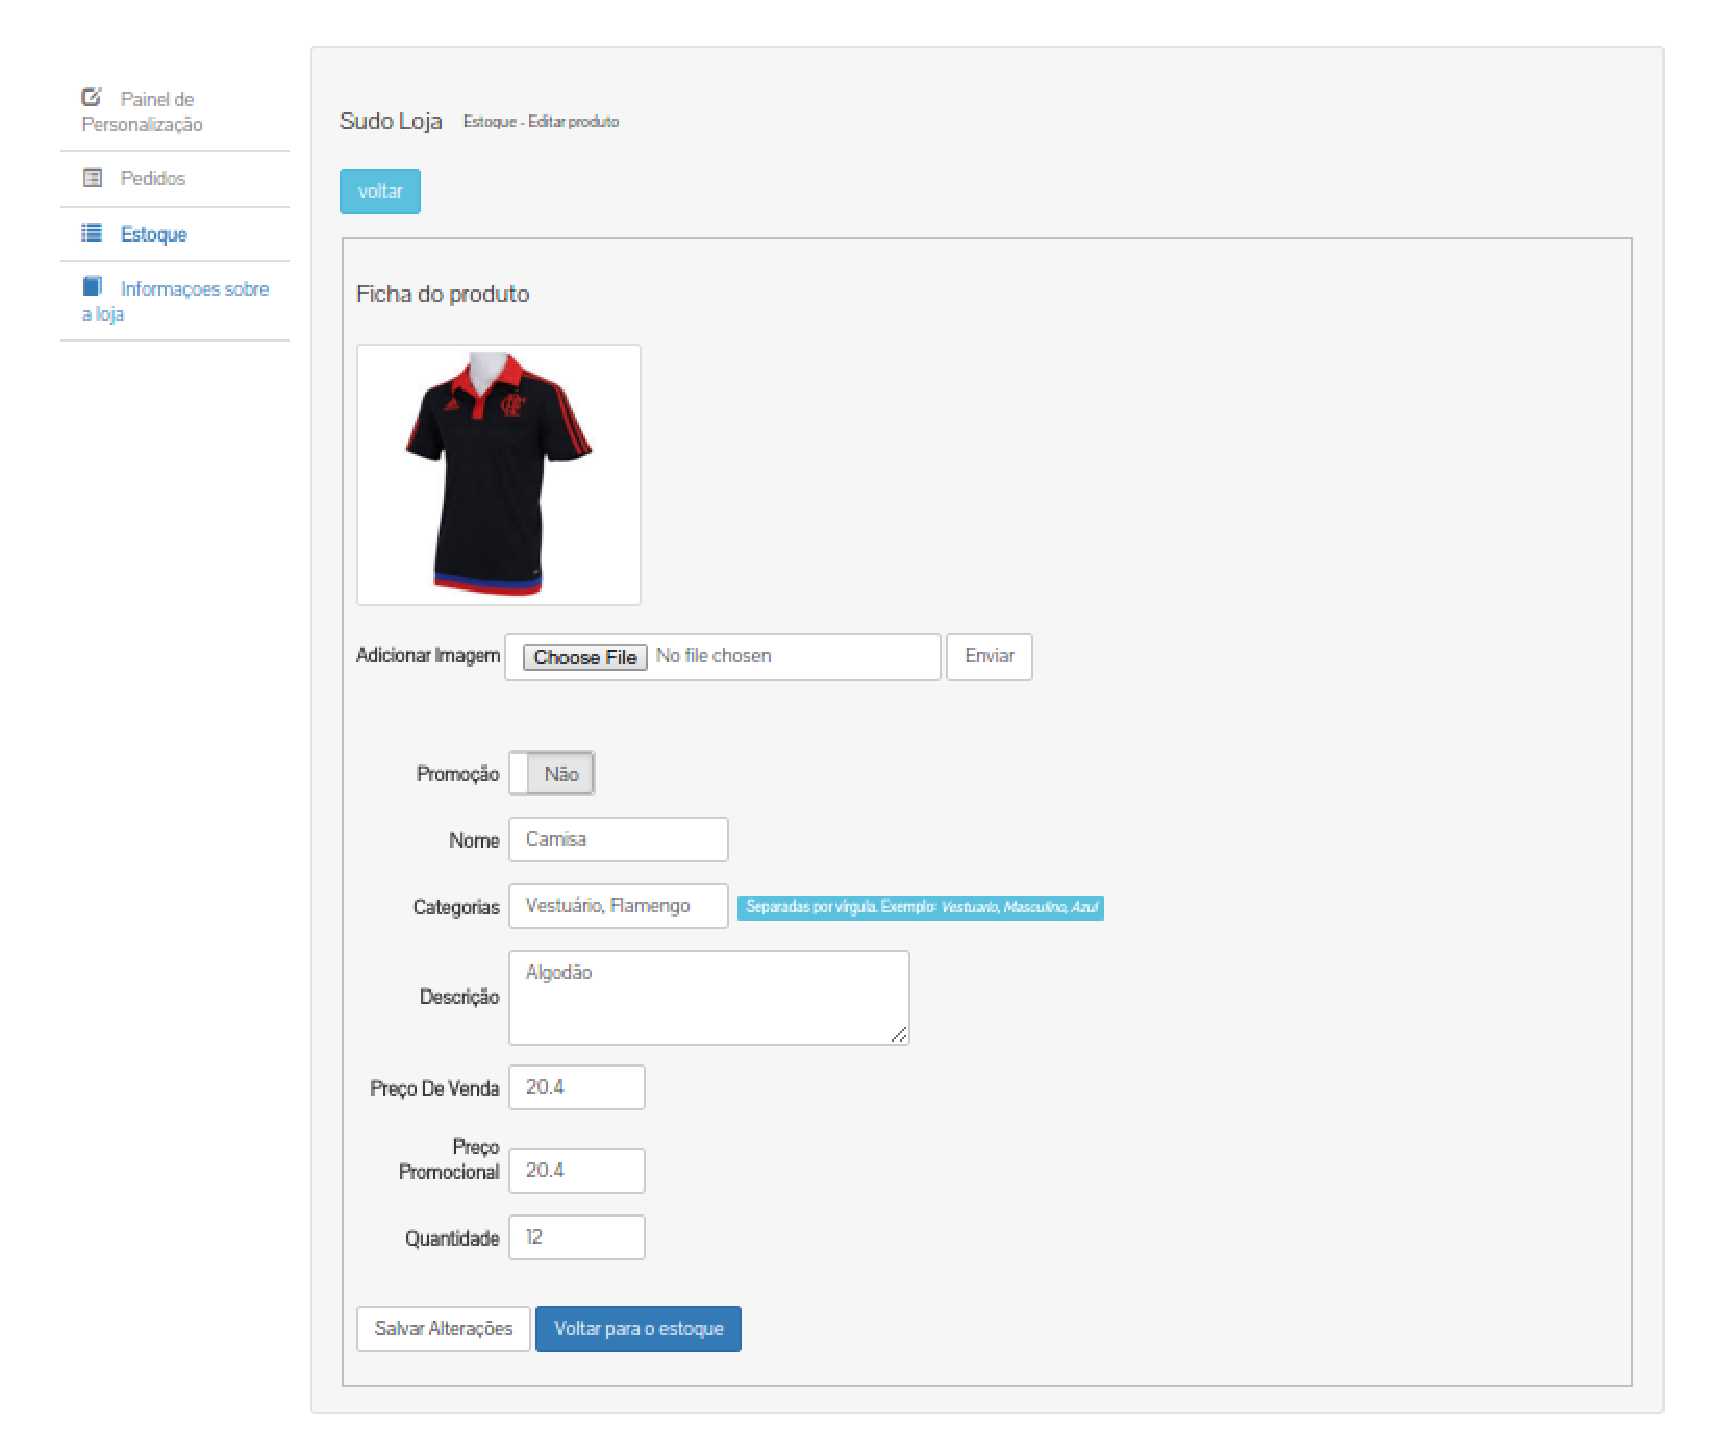
\includegraphics[width=15cm]{img/sistema/ficha-produto.eps}\\
\label{fig:ficha-produto}
\end{figure}

O estoque de uma loja do sistema é ilustrado na Figura \ref{fig:sistema-estoque}. Nessa página o usuário pode adicionar um novo produto, clicando no botão \textbf{Cadastrara novo produto}, onde será exibido um formulário para inserção dos dados do produto; Poderá também editar um produto, clicando sobre ele na tabela, sua ficha será exibida, onde o usuário poderá ver com detalhes todas as informações inerentes ao produto, podendo atualizá-las.

\vspace{1,5cm}
\begin{figure}[H]
\centering
\caption{Página do estoque de uma loja do sistema}
\centering
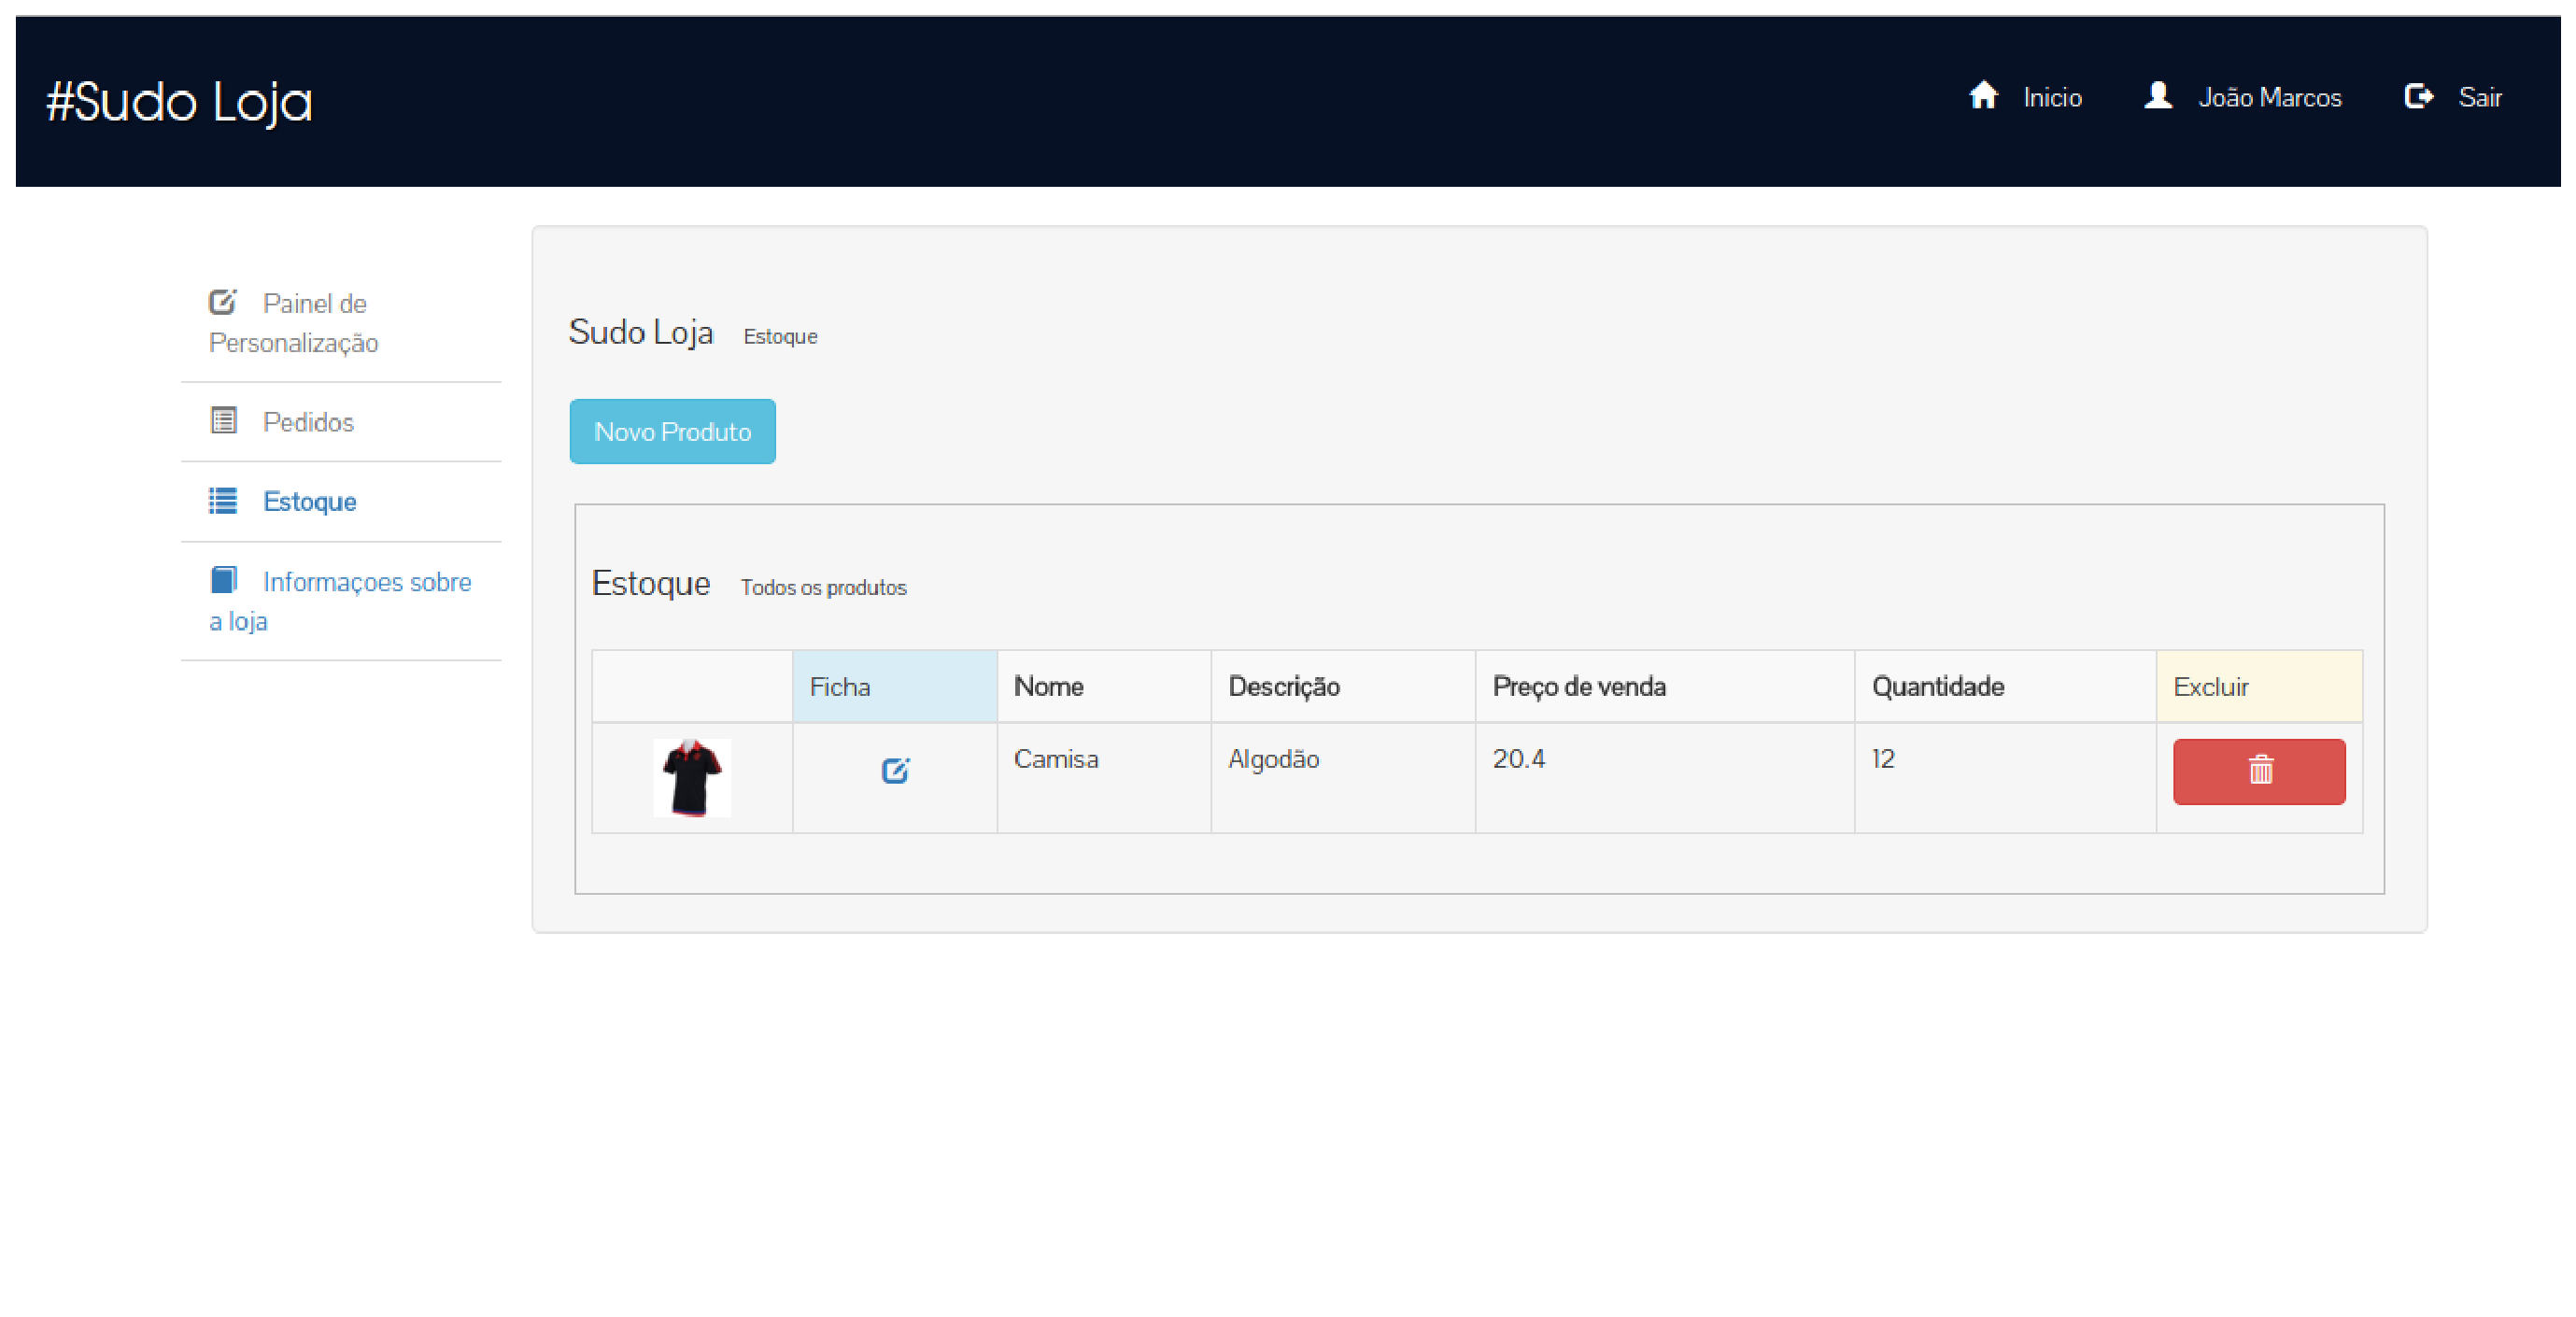
\includegraphics[width=15cm]{img/sistema/pagina-estoque.eps}\\
\label{fig:sistema-estoque}
\end{figure}


% section implementacao (end)
% chapter sudo_loja (end)

\chapter{Considerações Finais} % (fold)
\label{cha:considera_es_finais}

Para \citeonline{suh2002content}, um CMS busca automatizar o processo de criação, publicação e atualização de conteúdo em um web site. A Sudo Loja como sendo um CMS, automatiza uma série de tarefas quando se trata de criar uma loja virtual. O sistema torna a tarefa de criar, manter e atualizar o conteúdo de um \textit{e-commerce} mais fácil, e não apenas para usuários com algum conhecimento técnico. Aqueles cujo conhecimento seja considerado mínimo, poderá facilmente criar e introduzir conteúdo no seu site de vendas. 

Tudo isso feito a partir de um editor \textit{front-end}, por onde o usuário conseguirá abastecer sua loja com dados; um sistema \textit{back-end} para armazenar e processar o conteúdo; e um mecanismo que obtém o conteúdo e o renderiza, com base num modelo predefinido de site. Este modelo pode ser personalizado pelo próprio usuário, da mesma forma que acontece com o conteúdo.

Algumas tecnologias tiveram que ser abordadas com mais profundidade, para que o sistema pudesse ser finalizado e concluído como planejado. O Spring \textit{Framework}, por exemplo, tornou o desenvolvimento muito mais eficiente e rápido. O projeto foi iniciado sem o uso do Spring. Após sua integração notou-se maior velocidade e qualidade na confecção do código fonte.

\section{Trabalhos futuros} % (fold)
\label{sec:trabalhos_futuros}

O sistema desenvolvido trouxe um resultado satisfatório, porém alguns pontos ainda podem ser melhorados, e  novas funcionalidades poderiam ser acopladas.

\begin{itemize}
	\item O sistema utilizou apenas uma estratégia para a realização de pagamentos. O uso do PagSeguro, por ser gratuito. O pagamento direto na aplicação envolve custos para realizar a configuração e integração ao sistema. Essas plataformas poderiam ser integradas posteriormente, tornando o pagamento ainda mais amigável e rápido.
	\item A personalização foi feita a partir de um template pré definido. O sistema poderia disponibilizar a escolha dentre diversos templates.
	\item O sistema poderia possibilitar o uso de cupons de desconto em compras.
	\item O sistema poderia disponibilizar diferentes tipos de relatórios, como por exemplo, de vendas, ou produtos menos vendidos, entre outros.
\end{itemize}
% section trabalhos_futuros (end)
% chapter considera_es_finais (end)


					%----------------------- FIM DO DOCUMENTO ----------------------%
\bibliography{referencias}

% Inicio do Apêndice
\appendix
\newpage
\phantomsection
\addcontentsline{toc}{chapter}{Apêndices}  
\addtocontents{toc}{\protect\setcounter{tocdepth}{-1}}
\chapter{Documento de Visão}
\label{ap:documento_visao}
\section{Introdução} % (fold)
\label{sec:Introducao}

Este documento apresenta uma solução de software para ser apresentado como TCC, solicitado pelos professores. Como cliente Francisco Paulo de Freitas Neto (Orientador). Apresenta também os problemas a serem solucionados, as necessidades dos principais envolvidos, o alcance do projeto e as funcionalidades esperadas do sistema.

\subsection{Objetivos} % (fold)
\label{sec:objetivos}

Como objetivo principal, esse projeto visa facilitar o ingresso de um comerciante ao mercado virtual, fornecendo uma ferramenta capaz de criar uma loja virtual onde um usuário, sem ajuda especializada, poderá gerenciar e customizar sua loja de maneira simples e intuitiva.

% subsection objetivos (end)

\subsection{Abrangência do Projeto} % (fold)
\label{sec:abrengencia_do_projeto}

Esse projeto é voltado ao âmbito comercial, contemplando todos aqueles que desejam criar uma loja virtal e disponibilizar produtos à venda.
O produto final será uma plataforma onde qualquer usuário cadastrado poderá criar, gerenciar e personalizar uma loja virtual.

% subsection abrengencia_do_projeto (end)

\subsection{Definições, Acrônimos e Abreviações} % (fold)
\label{sec:siglas}

\textbf{CMS} – Content Management System (Sistema de Gerenciamento de Conteúdo)

% subsection siglas (end)
\subsection{Organização do Documento} % (fold)
\label{sec:organizacao_do_documento}

As próximas seções trataram sobre a descrição do problema, as partes envolvidas e tipos de usuários que utilizaram o sistema, a solução proposta para os problemas elencados, logo após, as funcionalidades oferecidas por esta solução, seguidas pelas restrições do sistema. Também poderão ser vistos alguns protótipos na Seção \ref{sec:prototipos}.

% subsection organizacao_do_documento (end)
% section Introdução (end)

\section{Descrição do Problema} % (fold)
\label{cha:descricao_do_problema}

\begin{itemize}
\item Dificuldades no gerenciamento de uma loja virtual - 
Aqueles que desejam entrar no mercado virtual geralmente recorrem a empresas de desenvolvimento de software para criar sua loja virtual, e geralmente, qualquer tipo de modificação a ser feita, seja no conteúdo ou no \textit{layout} e estilo do site, necessita da intervenção direta da equipe de desenvolvimento.

\item Afeta - O lojista.
\item O impacto deste problema é - 
Um grande impacto que isso causa para o lojista é a demora, tanto no desenvolvimento quanto na modificação de alguma parte da loja online, por exemplo, digamos que por algum motivo o lojista queira modificar o estilo do sua loja online. A equipe então, levará um certo tempo (dependendo da complexidade de modificação) até entender completamente o que o cliente deseja para então realizar a modificação e deixar a loja do jeito que o cliente pediu, e é claro, na maioria dos casos com um custo considerável. Então temos dois problemas principais: demora e custo.

\item Uma solução ideal permitiria - 
Fornecer um sistema que possibilitasse a criação, personalização  e gerenciamento de uma loja online sem intervenção de pessoal especializado, com um baixo custo.

\end{itemize}

% section descricao_do_problema (end)

\section{Partes Envolvidas} % (fold)
\label{sec:partes_envolvidas}

Os principais envolvidos serão descritos nas seções \ref{sec:resumo_dos_envolvidos} e \ref{sec:resumo_dos_usuarios}.

\subsection{Resumo dos Envolvidos} % (fold)
\label{sec:resumo_dos_envolvidos}

Os envolvidos que se interessam em empenhar-se nesse projeto, são os desenvolvedores, os comerciantes, e os consumidores.

% subsection resumo_dos_envolvidos (end)

\subsection{Resumo dos Usuários} % (fold)
\label{sec:resumo_dos_usuarios}

Uma lista resumida de todos os usuários identificados pode ser vista no Quadro \ref{quadro:usuarios}.

\begin{table}[H]
\centering
\caption{Resumo dos usuários}
\label{quadro:usuarios}
\begin{tabular*}{\textwidth}{@{\extracolsep{\fill}} |p{3cm}|p{4cm}|p{4cm}|p{3cm}|}
\hline
\rowcolor{ballblue}
Nome & 	Descrição & Responsabilidades & Envolvido \\
Lojista & Administrador da loja virtual &  Criação da loja, Personalização da loja, Inclusão de dados no sistema, Gerenciamento de pedidos 
& Dono do negócio ou alguém que represente seus interesses \\
\hline
Cliente & Consumidor dos produtos oferecidos na loja & Efetuar cadastro para realização de uma compra & Qualquer consumidor em potencial que deseje  realizar uma compra  (de um ou mais)  produtos oferecidos pela loja \\	
\hline
\end{tabular}
\end{table}

% subsection resumo_dos_usuarios (end)

% section partes_envolvidas (end)

\section{Descrição da Solução Proposta} % (fold)
\label{sec:descri_o_da_solu_o_proposta}

A solução proposta é um sistema computacional web para criação de lojas virtuais (um CMS voltado para criação de lojas, onde um usuário poderá criar, personalizar as suas lojas virtuais e assim, disponibilizar os seus produtos para venda) e uma área para perguntas ao vendedor sobre um produto desejado. tudo isso de forma simples sem conhecimento especializado, sem burocracias. 

% section descri_o_da_solu_o_proposta (end)

\section{Funcionalidades} % (fold)
\label{sec:funcionalidades}

No Quadro \ref{quadro:funcionalidades} podemos ver uma breve descrição das funcionalidades do produto, com um nível de detalhamento genérico para uma melhor compreensão.


\begin{longtable}{|p{7cm}|p{7cm}|}
\caption{Resumo das Funcionalidades}
\label{quadro:funcionalidades}
\hline
\rowcolor{ballblue}
Funcionalidade & Descrição	\\	
Gerenciamento de produtos & Inclusão, remoção e alteração de produtos, cadastro de múltiplas imagens para cada produto
\\	
\hline
Gerenciamento de pedidos & Controle de todos os pedidos realizados
\\	
\hline
Personalização da loja & A loja poderá ser personalizada totalmente (\textit{layout}, cores, fontes, edição de CSS e HTML)
\\	
\hline
Gerenciamento de clientes & Cadastro, alteração de dados cadastrais, remoção da conta.
\\	
\hline
Calculo de frete automático quando houver & Caso haja frete sobre um produto da loja, em tempo real o cliente poderá ver o valor do frete
\\	
\hline
Controle de estoque & O estoque poderá ser consultado e gerenciado, contendo opções como desabilitar/habilitar produtos, visualizar quantidade de cada produto, filtrar produtos por nome
\\	
\hline
Acompanhamento de pedidos para os clientes & Os clientes poderão visualizar o status do pedido a qualquer momento,
\\	
\hline
\end{longtable}	


% section funcionalidades (end)

\section{Restrições do Projeto} % (fold)
\label{sec:restricoes_do_projeto}

O sistema será uma aplicação WEB com design totalmente responsivo, o que significa que poderá ser utilizado tanto pelo navegador de um computador desktop, quanto pelo navegador do celular. Não possuirá restrições quanto ao sistema operacional utilizado pelo consumidor.

% section restricoes_do_projeto (end)

\section{Protótipos} % (fold)
\label{sec:prototipos}

\begin{figure}[H]
\centering
\caption{Visualização de produtos cadastrados}
\centering
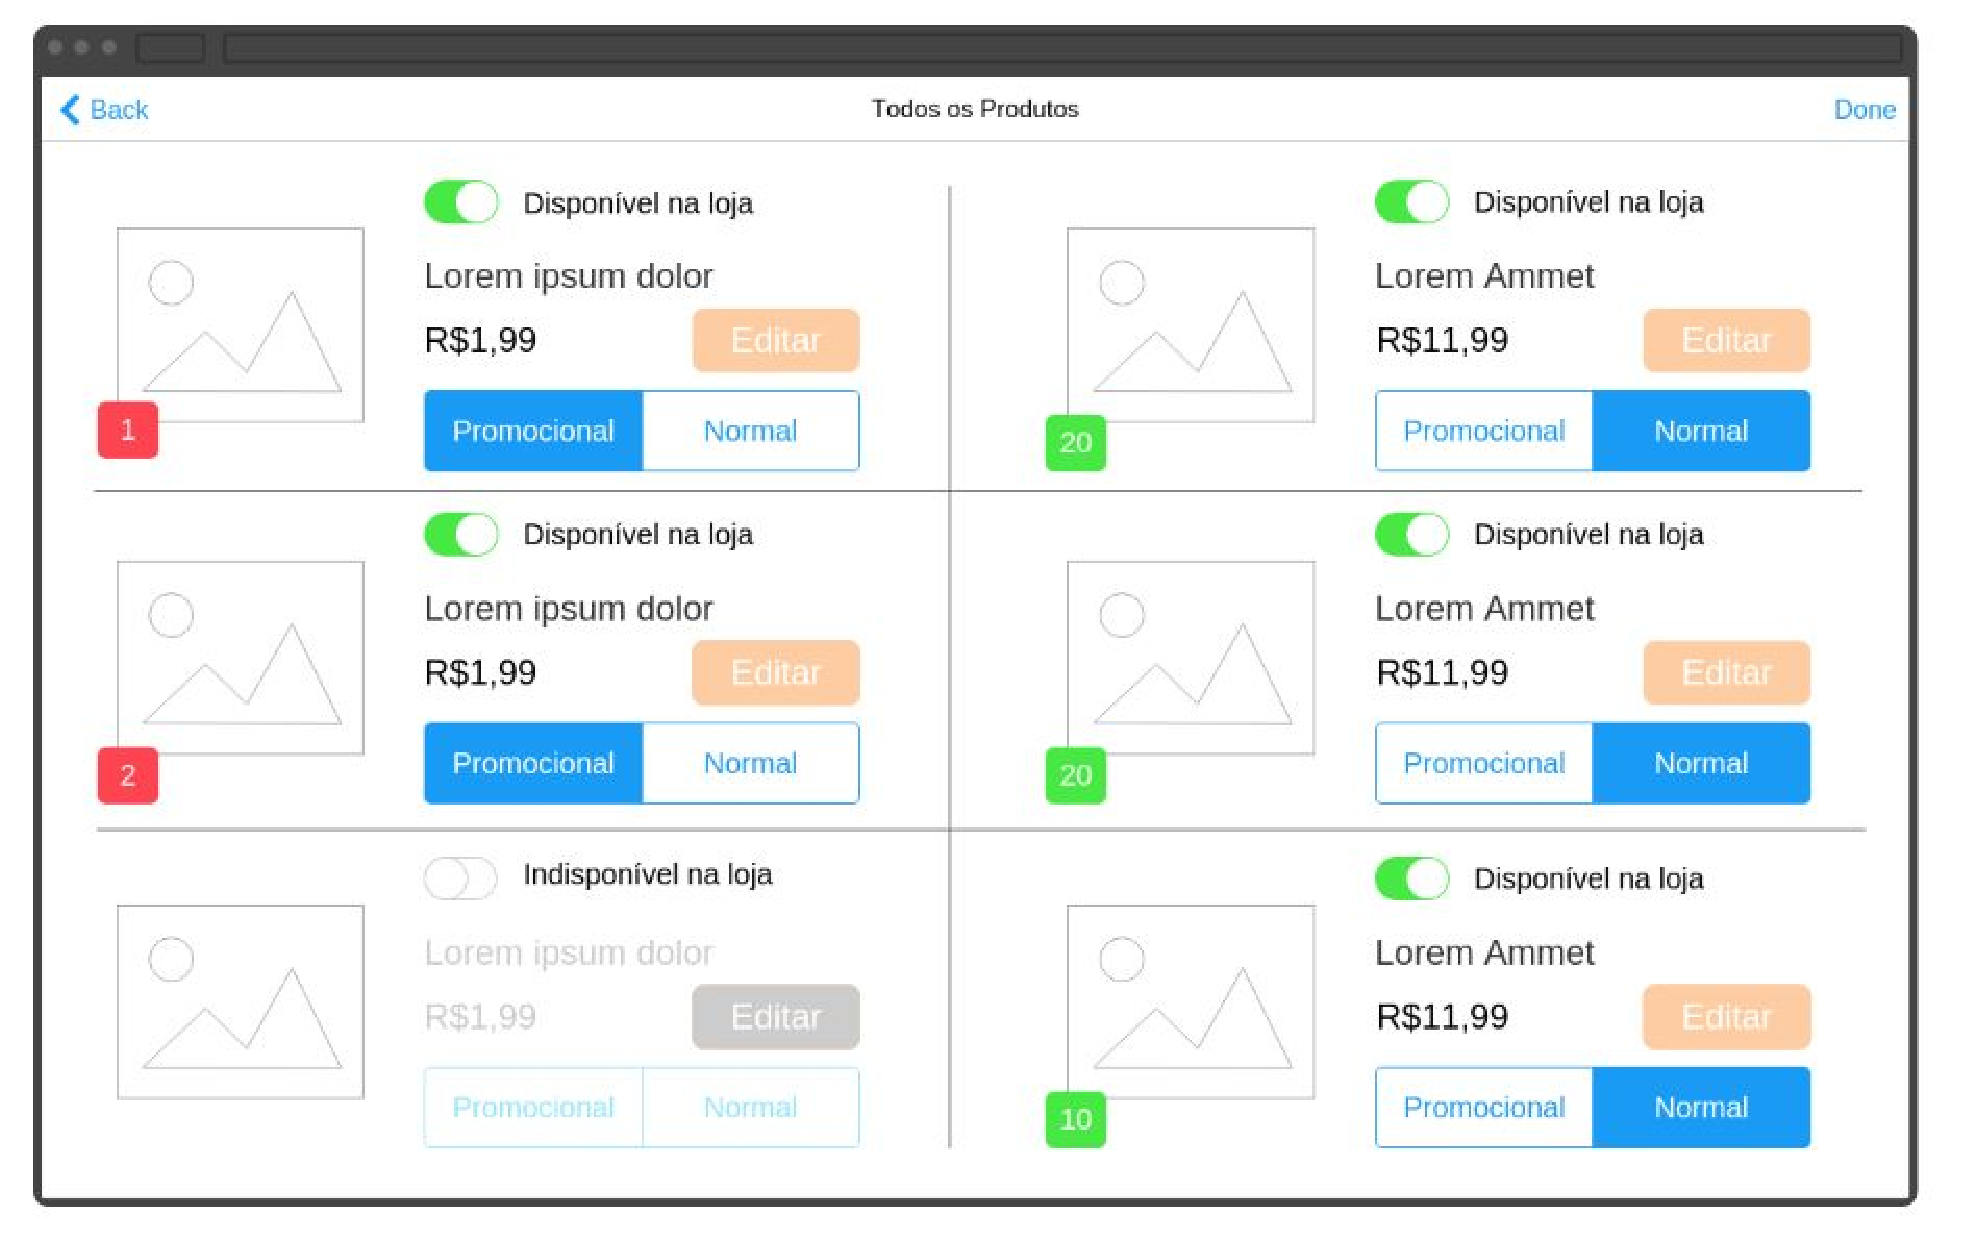
\includegraphics[width=12cm]{img/prototipos/produtos-cadastrados.eps}\\
\label{figura:produtos_cadastrados}
\end{figure}

\begin{figure}[H]
\centering
\caption{Cadastro de produtos}
\centering
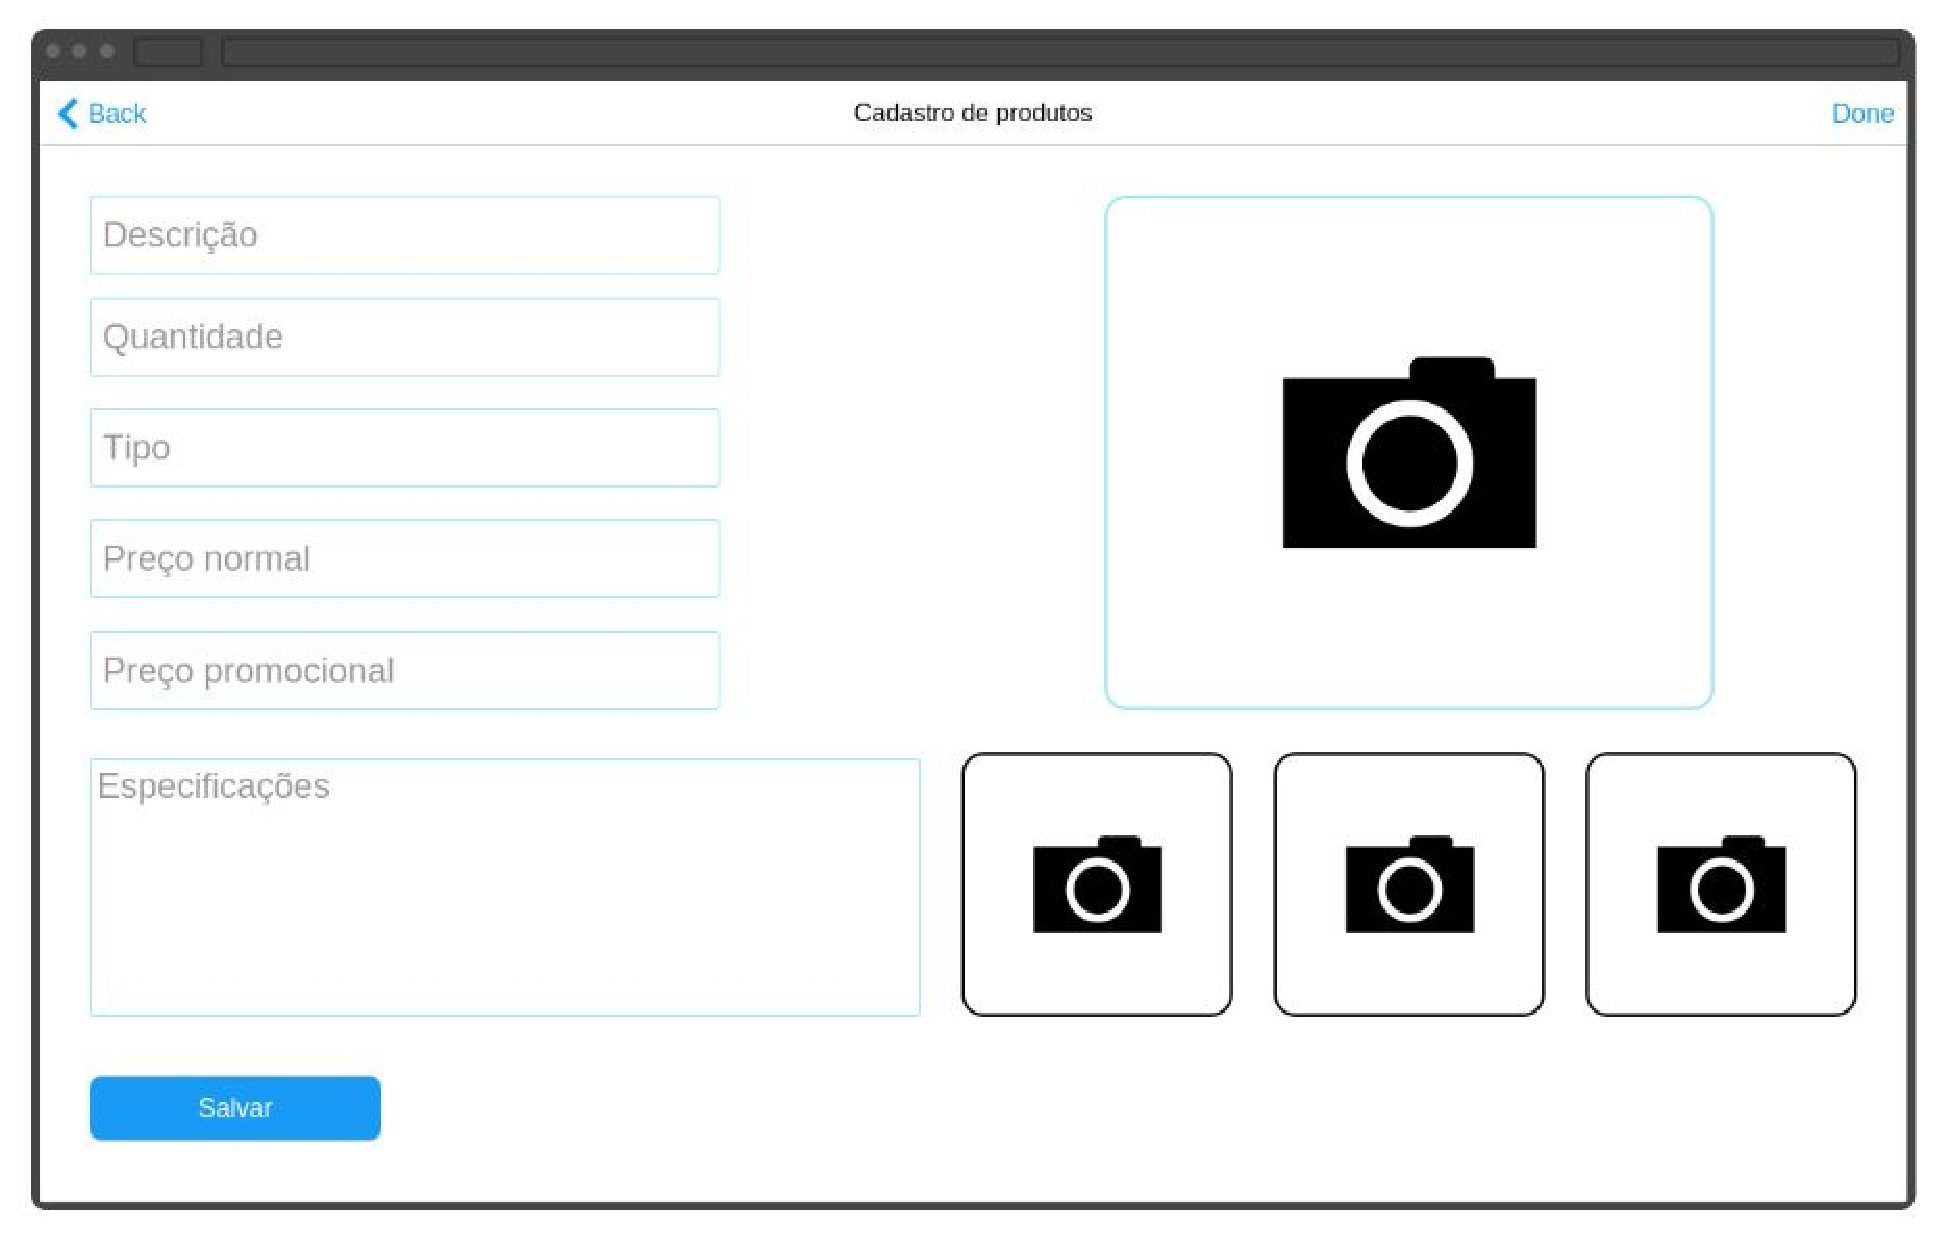
\includegraphics[width=12cm]{img/prototipos/cadastro-produto.eps}\\
\label{figura:Cadastro_de_Produtos}
\end{figure}

\begin{figure}[H]
\centering
\caption{Visualização de pedidos}
\centering
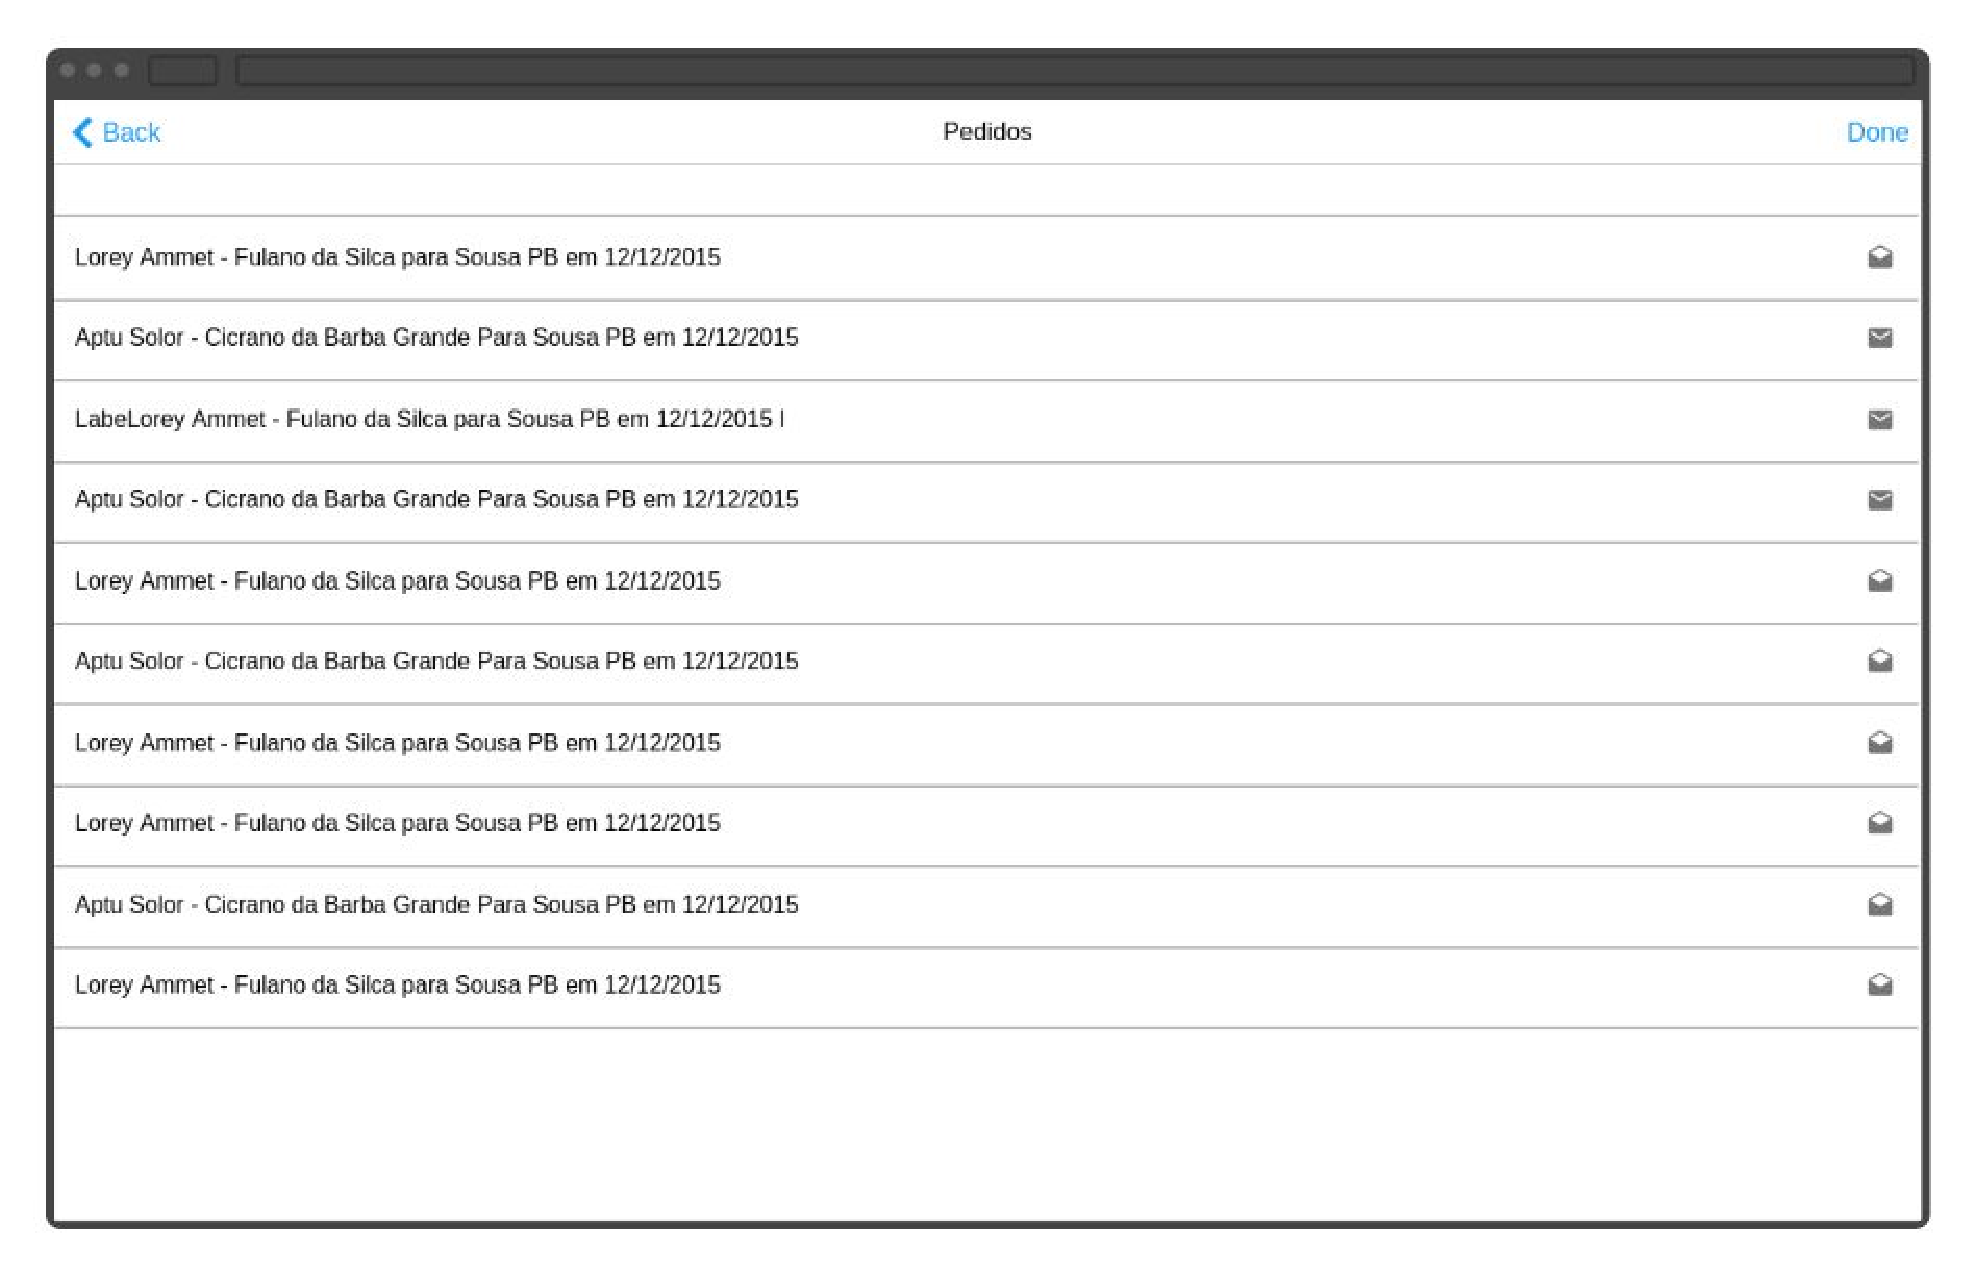
\includegraphics[width=12cm]{img/prototipos/visualizacao-pedido.eps}\\
\label{figura:visualizacao_pedidos}
\end{figure}

\begin{figure}[H]
\centering
\caption{Painel de Personalização}
\centering
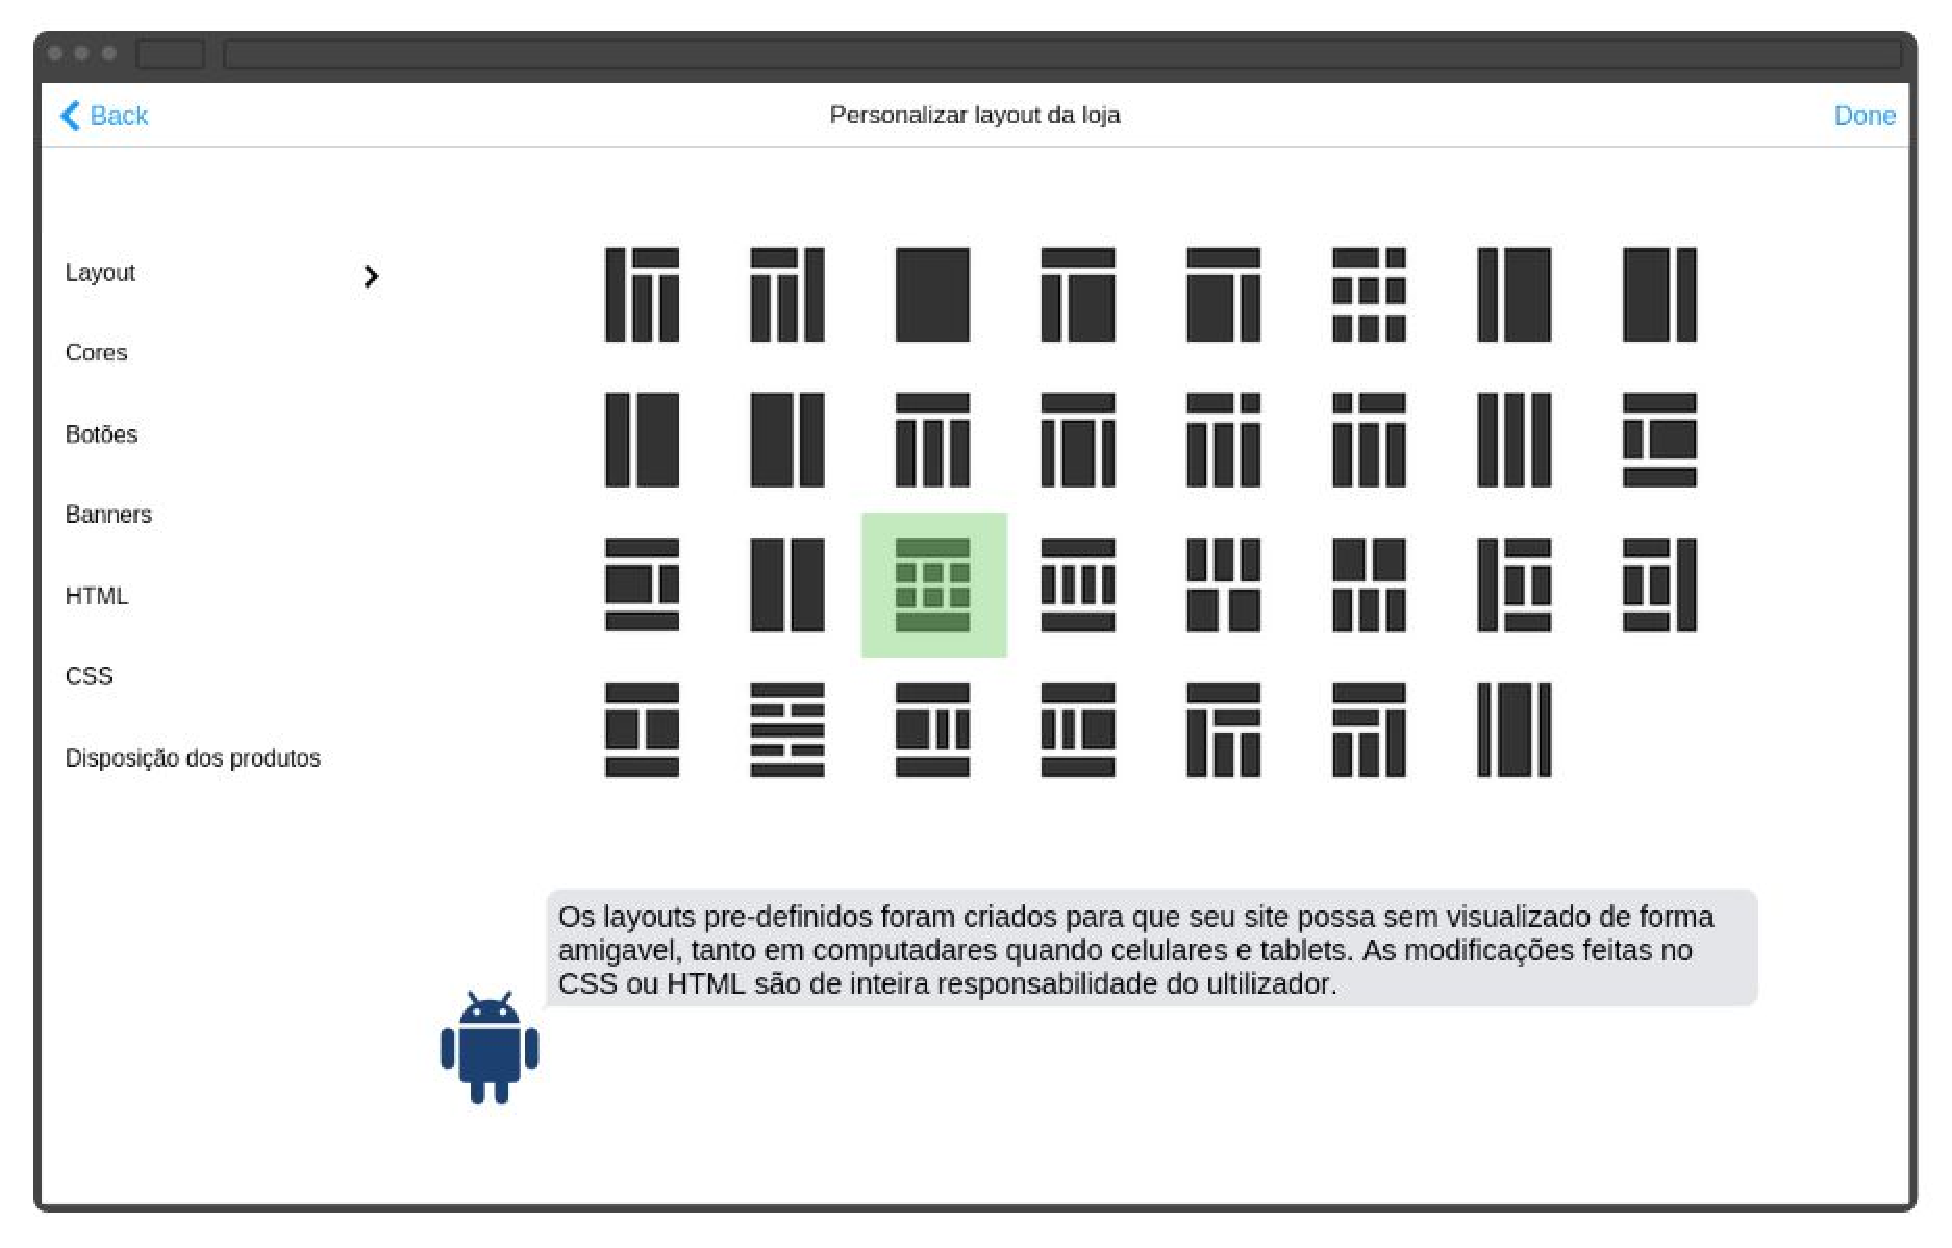
\includegraphics[width=12cm]{img/prototipos/painel-personalizacao.eps}\\
\label{figura:painel_personalizacao}
\end{figure}

\begin{figure}[H]
\centering
\caption{Controle de estoque}
\centering
\includegraphics[width=12cm]{img/prototipos/estoque.eps}\\
\label{figura:controle_estoque}
\end{figure}

% section prot_tipos (end)

\chapter{\textit{User Stories} e Testes de Aceitação} % (fold)
\label{app:user_stories_e_testes_de_aceitacao}

\begin{longtable}{|p{1.5cm}|p{3.5cm}|c|p{2cm}|p{2cm}|c|}
\caption{Alocação de Tarefas - US01}
\label{quadro:tat-us03}
\hline
\multicolumn{6}{|c|}{\textbf{\textit{User Story} 01}}\\
\hline		
\rowcolor{ballblue}
Tarefa & Descrição & Responsável & Estimativa de tempo (horas) & Tempo real (horas) & Status\\
\hline
T1 & Implementar Script para salvar um Usuário Lojista & João Marcos & 2 & 1 & Finalizado\\
\hline
T2 & Implementar Script para validar informações do usuário Lojista & João Marcos & 2 & 1 & Finalizado\\
\hline
T3 & Criar Formulário para cadastro usuários lojistas & João Marcos & 3 & 2 & Finalizado\\	
\hline
T5 & Criar página editar as informações do usuário Lojista & João Marcos & 4 & 3 & Finalizado\\	
\hline
\end{longtable}

\begin{longtable}{|l|p{11.8cm}|c|}
\caption{Teste de aceitação - US01}
\label{quadro:teste-aceitacao-us01}
\hline
\multicolumn{3}{|c|}{\textbf{\textit{User Story} 01}}\\
\hline		
\rowcolor{ballblue}
\multicolumn{2}{|c|}{Testes de aceitação} & Status\\	
\hline
TA1 & Dado que estou na página de registro de novo usuário, quando eu preencher o formulário com os dados obrigatórios de forma correta , o usuário deve ser salvo.   & Finalizado\\
\hline
TA2 & Dado que estou na página de registro de novo usuário, quando eu preencher o formulário com os dados obrigatórios de forma incorreta , o usuário não deve ser salvo e uma mensagem de erro deve ser exibida.   & Finalizado\\
\hline
TA3 & Dado que estou acessando a ficha de edição de informações sobre o Lojista, quando eu alterar alguma informação do formulário com os dados válidos, o usuário deve ser atualizado e uma mensagem de sucesso deve ser exibida.   & Finalizado\\
\hline
TA4 & Dado que estou acessando a ficha de edição de informações sobre o Lojista, quando eu alterar alguma informação do formulário com os dados inválidos, tais informações não serão salvas e uma mensagem de erro deve ser exibida.   & Finalizado\\
\hline	
\end{longtable}

\begin{longtable}{|p{1.5cm}|p{3.5cm}|c|p{2cm}|p{2cm}|c|}
\caption{Alocação de Tarefas - US01}
\label{quadro:tat-us03}
\hline
\multicolumn{6}{|c|}{\textbf{\textit{User Story} 02}}\\
\hline		
\rowcolor{ballblue}
Tarefa & Descrição & Responsável & Estimativa de tempo (horas) & Tempo real (horas) & Status\\
\hline
T1 & Implementar Script para salvar uma Loja & João Marcos & 2 & 1 & Finalizado\\
\hline
T2 & Implementar Script para validar informações do de uma Loja & João Marcos & 2 & 1 & Finalizado\\
\hline
T3 & Criar Formulário para cadastro de uma Loja & João Marcos & 3 & 2 & Finalizado\\	
\hline
T5 & Criar página editar as informações Sobre uma Loja & João Marcos & 4 & 3 & Finalizado\\
\hline
\end{longtable}

\begin{longtable}{|l|p{11.8cm}|c|}
\caption{Teste de aceitação - US02}
\label{quadro:teste-aceitacao-us02}
\hline
\multicolumn{3}{|c|}{\textbf{\textit{User Story} 02}}\\
\hline		
\rowcolor{ballblue}
\multicolumn{2}{|c|}{Testes de aceitação} & Status\\	
\hline
TA1 & Dado que estou na página de criação de uma Loja, quando eu preencher o formulário com os dados obrigatórios de forma correta , a loja ser salva.   & Finalizado\\
\hline
TA2 & Dado que estou na página criação de uma Loja, quando eu preencher o formulário com os dados obrigatórios de forma incorreta , a Loja não deve ser salva e uma mensagem de erro deve ser exibida.   & Finalizado\\
\hline
TA3 & Dado que estou acessando a página de edição de informações sobre uma Loja, quando eu alterar alguma informação do formulário com os dados válidos, a Loja deve ser atualizada e uma mensagem de sucesso deve ser exibida.   & Finalizado\\
\hline
TA4 & Dado que estou acessando a página de edição de informações sobre uma Loja, quando eu alterar alguma informação do formulário com os dados inválidos, tais informações não serão salvas e uma mensagem de erro deve ser exibida.   & Finalizado\\
\hline	
TA5 & Permitir que eu possa cadastrar mais de uma Loja no sistema.  & Finalizado\\
\hline	
\end{longtable}

\begin{longtable}{|p{1.5cm}|p{3.5cm}|c|p{2cm}|p{2cm}|c|}
\caption{Alocação de Tarefas - US03}
\label{quadro:tat-us03}
\hline
\multicolumn{6}{|c|}{\textbf{\textit{User Story} 03}}\\
\hline		
\rowcolor{ballblue}
Tarefa & Descrição & Responsável & Estimativa de tempo (horas) & Tempo real (horas) & Status\\
\hline
T1 & Implementar Script para salvar um Produto & João Marcos & 2 & 1 & Finalizado\\
\hline
T2 & Implementar Script para validar informações do produto & João Marcos & 2 & 1 & Finalizado\\
\hline
T3 & Criar Formulário para cadastro de produto & João Marcos & 3 & 2 & Finalizado\\
\hline
T4 & Criar formulário para edição de produto & João Marcos & 2 & 1 & Finalizado\\
\hline
T5 & Criar página para o estoque, exibindo as informações básicas de cada produto com sua respectiva quantidade e link para ficha do produto & João Marcos & 4 & 3 & Finalizado\\
\hline
T6 & Criar botão para exclusão de um produto na página de estoque & João Marcos & 2 & 1 & Finalizado\\
\hline
\end{longtable}

\begin{longtable}{|l|p{11.8cm}|c|}
\caption{Teste de aceitação - US03}
\label{quadro:teste-aceitacao-us03}
\hline
\multicolumn{3}{|c|}{\textbf{\textit{User Story} 03}}\\
\hline		
\rowcolor{ballblue}
\multicolumn{2}{|c|}{Testes de aceitação} & Status\\	
\hline
TA1 & Dado que estou na página de cadastro de produto, quando eu preencher o formulário com os dados obrigatórios de forma correta , o produto deve ser salvo e informado uma mensagem de sucesso.   & Finalizado\\
\hline
TA2 & Dado que estou na página de cadastro de produto, quando eu preencher o formulário com os dados obrigatórios de forma incorreta , o produto não deve ser salvo e uma mensagem de erro deve ser exibida.   & Finalizado\\
\hline
TA3 & Dado que estou acessando a ficha de edição de produto, quando eu alterar alguma informação do formulário com os dados válidos, o produto deve ser atualizado e uma mensagem de sucesso deve ser exibida.   & Finalizado\\
\hline
TA4 & Dado que estou acessando a ficha de edição de produto, quando eu alterar alguma informação do formulário com os dados inválidos, tais informações não serão salvas e uma mensagem de erro deve ser exibida.   & Finalizado\\
\hline
TA5 & Dado que estou na página de estoque, quando eu selecionar a opção excluir este produto, um diálogo de confirmação deve ser exibido. Caso confirme o produto deve ser excluído  & Finalizado\\
\hline
TA6 & Dado que estou na página de estoque, quando eu selecionar a opção excluir este produto, um diálogo de confirmação deve ser exibido. Caso não confirme o produto não deve ser excluído  & Finalizado\\
\hline
\end{longtable}

\begin{longtable}{|p{1.5cm}|p{3.5cm}|c|p{2cm}|p{2cm}|c|}
\caption{Alocação de Tarefas - US04}
\label{quadro:tat-us04}
\hline
\multicolumn{6}{|c|}{\textbf{\textit{User Story} 04}}\\
\hline		
\rowcolor{ballblue}
Tarefa & Descrição & Responsável & Estimativa de tempo (horas) & Tempo real (horas) & Status\\
\hline
T1 & Implementar Script para validar credenciais de um lojista & João Marcos & 2 & 1 & Finalizado\\
\hline
T2 & Criar página inicial contendo um menu de navegação onde o usuário poderá navegar com facilidade no sistema & João Marcos & 4 & 3 & Finalizado\\
\hline
T3 & Criar botão para sair do Sistema & João Marcos & 2 & 1 & Finalizado\\
\hline
T4 & Criar página de seleção de lojas, onde o usuário poderá escolher a loja que deseja gerenciar no momento & João Marcos & 5 & 4 & Finalizado\\
\hline
T5 & Criar página de gerenciamento específica para lojas, que será exibida ao selecionar uma Loja na T4 & João Marcos & 4 & 2 & Finalizado\\
\hline
T6 & Criar menu lateral na página de gerenciamento da loja, permitindo a navegação dentre as funcionalidades inerentes ao gerenciamento da loja & João Marcos & 2 & 1 & Finalizado\\
\hline
\end{longtable}

\begin{longtable}{|l|p{11.8cm}|c|}
\caption{Teste de aceitação - US04}
\label{quadro:teste-aceitacao-us04}
\hline
\multicolumn{3}{|c|}{\textbf{\textit{User Story} 04}}\\
\hline		
\rowcolor{ballblue}
\multicolumn{2}{|c|}{Testes de aceitação} & Status\\	
\hline
TA1 & Dado que estou na página de login, quando eu preencher o formulário com os dados obrigatórios de forma correta , ser redirecionado para a página inicial do sistema.   & Finalizado\\
\hline
TA2 & Dado que estou na página de login, quando eu preencher o formulário com os dados obrigatórios de forma incorreta , não posso ser redirecionado para o sistema e uma mensagem de erro deve ser exibida.   & Finalizado\\
\hline
TA3 & Dado que estou logado, quando clicar no botão sair, devo ser desconectado do sistema, onde terei que fazer login novamente caso queira entrar no sistema novamente.   & Finalizado\\
\hline
TA4 & Dado que estou na página de seleção de lojas, quando selecionar uma loja, devo ser redirecionado  para página inicial de gerenciamento da Loja selecionada.  & Finalizado\\
\hline
TA5 & Dado que estou logado, quando eu selecionar uma opção do menu lateral, devo ser redirecionado para página especificada  & Finalizado\\
\hline	
\end{longtable}

\begin{longtable}{|p{1.5cm}|p{3.5cm}|c|p{2cm}|p{2cm}|c|}
\caption{Alocação de Tarefas - US05}
\label{quadro:tat-us05}
\hline
\multicolumn{6}{|c|}{\textbf{\textit{User Story} 05}}\\
\hline		
\rowcolor{ballblue}
Tarefa & Descrição & Responsável & Estimativa de tempo (horas) & Tempo real (horas) & Status\\
\hline
T1 & Implementar Script para salvar preferência & João Marcos & 2 & 1 & Finalizado\\
\hline
T2 & Classificar alterações com base na seção da página e as expor em um menu lateral & João Marcos & 2 & 1 & Finalizado\\
\hline
T3 & Criar formulário para cada tipo de modificação na aparência do site & João Marcos & 5 & 3 & Finalizado\\
\hline
T4 & Criar alerta ao salvar um alteração & João Marcos & 2 & 1 & Finalizado\\
\hline
T4 & Criar botão para reverter configurações para padrões & João Marcos & 2 & 1 & Finalizado\\
\hline
\end{longtable}

\begin{longtable}{|l|p{11.8cm}|c|}
\caption{Teste de aceitação - US05}
\label{quadro:teste-aceitacao-us05}
\hline
\multicolumn{3}{|c|}{\textbf{\textit{User Story} 05}}\\
\hline		
\rowcolor{ballblue}
\multicolumn{2}{|c|}{Testes de aceitação} & Status\\	
\hline
TA1 & Dado que estou logado no sistema, quando eu selecionar uma loja, o menu de personalização referente a essa loja é carregado  & Finalizado\\
\hline
TA2 & Dado que selecionei uma seção no menu de personalização, um conjunto de formulário inerentes a esta é carregado e exibido ao utilizador.   & Finalizado\\
\hline
TA3 & Dado que alterei o estilo de algo usando o formulário, ao clicar em salvar, as alterações devem ser salvas.   & Finalizado\\
\hline
TA4 & Dado que retornei a uma seção de menu de personalizações já alterada, a mesma deve carregar as preferencias anteriormente salvas.  & Finalizado\\
\hline
TA5 & Dado que cliquei no botão ``reverter alterações'' as modificações devem ser ignoradas e as configurações padrões aplicadas  & Finalizado\\
\hline
\end{longtable}


\begin{longtable}{|p{1.5cm}|p{3.5cm}|c|p{2cm}|p{2cm}|c|}
\caption{Alocação de Tarefas - US06}
\label{quadro:tat-us06}
\hline
\multicolumn{6}{|c|}{\textbf{\textit{User Story} 06}}\\
\hline		
\rowcolor{ballblue}
Tarefa & Descrição & Responsável & Estimativa de tempo (horas) & Tempo real (horas) & Status\\
\hline
T1 & Implementar Script para salvar usuário da loja & João Marcos & 2 & 1 & Finalizado\\
\hline
T2 & Criar página para cadastro/login de cliente de uma loja & João Marcos & 3 & 3 & Finalizado\\
\hline
T3 & Criar página para visualização de usuários para cada loja & João Marcos & 2 & 1 & Finalizado\\
\end{longtable}

\begin{longtable}{|l|p{11.8cm}|c|}
\caption{Teste de aceitação - US06}
\label{quadro:teste-aceitacao-us06}
\hline
\multicolumn{3}{|c|}{\textbf{\textit{User Story} 06}}\\
\hline		
\rowcolor{ballblue}
\multicolumn{2}{|c|}{Testes de aceitação} & Status\\	
\hline
TA1 & Dado que estou na página de cadastro, ao informar e-mail e senha corretos devo ser redirecionado para a página principal da loja & Finalizado\\
\hline
TA2 & Quando clicar no botão ``sair'' minha seção seja encerrada e devo ser redirecionado para a página inicial  & Finalizado\\
\hline
TA3 & Dado que estou no painel de controle, ao selecionar a opção ``usuários'' a lista de usuários cadastrado em minha loja deve ser exibida.   & Finalizado\\
\hline
\end{longtable}


\begin{longtable}{|p{1.5cm}|p{3.5cm}|c|p{2cm}|p{2cm}|c|}
\caption{Alocação de Tarefas - US07}
\label{quadro:tat-us07}
\hline
\multicolumn{6}{|c|}{\textbf{\textit{User Story} 07}}\\
\hline		
\rowcolor{ballblue}
Tarefa & Descrição & Responsável & Estimativa de tempo (horas) & Tempo real (horas) & Status\\
\hline
T1 & Implementar Script para carregamento de pedidos de cliente & João Marcos & 2 & 2 & Finalizado\\
\hline
T2 & Criar página para visualização de pedidos e informações básicas do cliente & João Marcos & 5 & 3 & Finalizado\\
\hline
T3 & Criar quadros expansíveis para cada pedido & João Marcos & 2 & 1 & Finalizado\\
\hline
T4 & Sinalizar status de cada pedido & João Marcos & 2 & 1 & Finalizado\\
\hline
\end{longtable}

\begin{longtable}{|l|p{11.8cm}|c|}
\caption{Teste de aceitação - US07}
\label{quadro:teste-aceitacao-us07}
\hline
\multicolumn{3}{|c|}{\textbf{\textit{User Story} 07}}\\
\hline		
\rowcolor{ballblue}
\multicolumn{2}{|c|}{Testes de aceitação} & Status\\	
\hline
TA1 & Dado que estou na página de acompanhamento, devo visualizar minhas informações e informações sobre pedidos feitos por mim.\\
\hline
TA2 & Dado que estou na página de acompanhamento, quando eu clicar em um pedido, o mesmo deve ser expandido e exibir seus detalhes e seu andamento, juntamente com um código de referência   & Finalizado\\
\hline
TA3 & Dado que expandi um pedido, ao clicar na imagem de um produto, devo ser levado até a sua página para que o mesmo seja exibido em detalhes.   & Finalizado\\
\hline
\end{longtable}


\begin{longtable}{|p{1.5cm}|p{3.5cm}|c|p{2cm}|p{2cm}|c|}
\caption{Alocação de Tarefas - US08}
\label{quadro:tat-us08}
\hline
\multicolumn{6}{|c|}{\textbf{\textit{User Story} 08}}\\
\hline		
\rowcolor{ballblue}
Tarefa & Descrição & Responsável & Estimativa de tempo (horas) & Tempo real (horas) & Status\\
\hline
T1 & Implementar Script para salvar pergunta sobre determinado produto & João Marcos & 5 & 2 & Finalizado\\
\hline
T2 & Criar página para visualização perguntas e respostas, classificadas por data e hora & João Marcos & 5 & 3 & Finalizado\\
\hline
T3 & Criar formulário para submeter pergunta & João Marcos & 2 & 1 & Finalizado\\
\hline
T4 & Alertar lojista sobre novas perguntas & João Marcos & 2 & 1 & Finalizado\\
\hline
\end{longtable}

\begin{longtable}{|l|p{11.8cm}|c|}
\caption{Teste de aceitação - US08}
\label{quadro:teste-aceitacao-us08}
\hline
\multicolumn{3}{|c|}{\textbf{\textit{User Story} 08}}\\
\hline		
\rowcolor{ballblue}
\multicolumn{2}{|c|}{Testes de aceitação} & Status\\	
\hline
TA1 & Dado que estou logado como usuário de loja, devo poder fazer quantas perguntas quiser sobre determinado produto em sua página & Finalizado\\
\hline
TA2 & Dado que submeti um pergunta, a mesma deve ser salva e alertada ao lojista  & Finalizado\\
\hline
TA3 & Dado que sou um lojista logado no sistema, ao perceber uma nova pergunta poderei respondê-la e a resposta deve aparecer junto a pergunta feita pelo usuário na página do produto   & Finalizado\\
\hline
\end{longtable}


\begin{longtable}{|p{1.5cm}|p{3.5cm}|c|p{2cm}|p{2cm}|c|}
\caption{Alocação de Tarefas - US09}
\label{quadro:tat-us09}
\hline
\multicolumn{6}{|c|}{\textbf{\textit{User Story} 09}}\\
\hline		
\rowcolor{ballblue}
Tarefa & Descrição & Responsável & Estimativa de tempo (horas) & Tempo real (horas) & Status\\
\hline
T1 & Alertar lojista sobre endereço não cadastrado & João Marcos & 1 & 1 & Finalizado\\
\hline
T2 & Definir endereço padrão de origem dos produto & João Marcos & 2 & 1 & Finalizado\\
\hline
T3 & Implementar script para consulta frete SEDEX e PAC & João Marcos & 3 & 3 & Finalizado\\
\hline
T4 & Adicionar campo peso ao produto, e botão para definir se este é passível ao cálculo de frete ou não & João Marcos & 2 & 1 & Finalizado\\
\hline
T5 & Implementar script para simular valor de frete a partir de um CEP informado & João Marcos & 2 & 1 & Finalizado\\
\hline
T6 & Criar formulário para simulação de frete & João Marcos & 2 & 1 & Finalizado\\
\hline
T7 & Listar e selecionar automaticamente o ultimo endereço informado pelo cliente em uma compra e calcular o frete com base nele & João Marcos & 2 & 1 & Finalizado\\
\hline
T8 & Página para alternar entre endereços já usados pelo usuário & João Marcos & 2 & 1 & Finalizado\\
\hline
T9 & Opção de escolha para frete, entre SEDEX e PAC & João Marcos & 2 & 1 & Finalizado\\
\hline
\end{longtable}

\begin{longtable}{|l|p{11.8cm}|c|}
\caption{Teste de aceitação - US09}
\label{quadro:teste-aceitacao-us09}
\hline
\multicolumn{3}{|c|}{\textbf{\textit{User Story} 09}}\\
\hline		
\rowcolor{ballblue}
\multicolumn{2}{|c|}{Testes de aceitação} & Status\\	
\hline
TA1 & Dado que estou na página do carrinho da loja, e este contenha algum item, um formulário de simulação de frete deve ser exibido & Finalizado\\
\hline
TA2 & Ao informar um CEP válido para simulação o resultado deve ser apresentado junto ao valor total do carrinho  & Finalizado\\
\hline
TA3 & Ao informar um CEP inválido para simulação o usuário deve ser alertado sobre isso  & Finalizado\\
\hline
TA4 & Dado que submeti um CEP para simulação do valor de entrega, e este seja válido, quando os produtos não possuírem frete, a palavra ``Grátis'' é exibida no local onde seria exibido o valor do frete  & Finalizado\\
\hline
TA5 & Dado que estou na página de checkout, o frete deve ser automaticamente calculado com base no ultimo endereço informado pelo usuário  & Finalizado\\
\hline
TA6 & Dado que conclui um pedido, as informações de frete devem ser exibidas na página de acompanhamento de pedidos  & Finalizado\\
\hline
TA7 & Ao tentar calcular o frete, sinalizar de alguma forma o andamento do processamento & Finalizado\\
\hline
\end{longtable}

\begin{longtable}{|p{1.5cm}|p{3.5cm}|c|p{2cm}|p{2cm}|c|}
\caption{Alocação de Tarefas - US10}
\label{quadro:tat-us10}
\hline
\multicolumn{6}{|c|}{\textbf{\textit{User Story} 10}}\\
\hline		
\rowcolor{ballblue}
Tarefa & Descrição & Responsável & Estimativa de tempo (horas) & Tempo real (horas) & Status\\
\hline
T1 & Implementar script para salvar imagens & João Marcos & 2 & 1 & Finalizado\\
\hline
T2 & Implementar script para atualizar imagens & João Marcos & 2 & 1 & Finalizado\\
\hline
T3 & Criar formulário para inserção e modificação das imagens de um produto & João Marcos & 3 & 1 & Finalizado\\
\hline
T4 & Criar uma galeria na página do produto, com as imagens cadastradas para o mesmo & João Marcos & 4 & 3 & Finalizado\\
\hline
T5 & Alternar imagem em destaque na galeria através de clique & João Marcos & 2 & 1 & Finalizado\\
\hline
\end{longtable}

\begin{longtable}{|l|p{11.8cm}|c|}
\caption{Teste de aceitação - US10}
\label{quadro:teste-aceitacao-us10}
\hline
\multicolumn{3}{|c|}{\textbf{\textit{User Story} 10}}\\
\hline		
\rowcolor{ballblue}
\multicolumn{2}{|c|}{Testes de aceitação} & Status\\	
\hline
TA1 & Dado que estou na página do produto, a galeria deve ser exibida com suas imagens & Finalizado\\
\hline
TA2 & Ao clicar em uma imagem da galeria a mesma dever ficar em destaque  & Finalizado\\
\hline
TA3 & O número de imagens para cada produto não pode passar de 5 (cinco)  & Finalizado\\
\hline
TA4 & O formato e o tamanho das imagens devem ser filtrados antes de sua inserção  & Finalizado\\
\hline
TA5 & Caso cadastre uma imagem não válida devo ser informado disso através de um alerta  & Finalizado\\
\hline
\end{longtable}
% chapter user_stories_e_testes_de_aceita_o (end)


\begin{longtable}{|p{1.5cm}|p{3.5cm}|c|p{2cm}|p{2cm}|c|}
\caption{Alocação de Tarefas - US11}
\label{quadro:tat-us11}
\hline
\multicolumn{6}{|c|}{\textbf{\textit{User Story} 11}}\\
\hline		
\rowcolor{ballblue}
Tarefa & Descrição & Responsável & Estimativa de tempo (horas) & Tempo real (horas) & Status\\
\hline
T1 & Implementar script realizar pagamento (integração PagSeguro) & João Marcos & 5 & 4 & Finalizado\\
\hline
T2 & Implementar script para salvar dados de pagamento (PagSeguro) & João Marcos & 1 & 1 & Finalizado\\
\hline
T3 & Criar formulário para inserção de dados de pagamento no painel administrativo & João Marcos & 2 & 1 & Finalizado\\
\hline
T4 & Criar página para visualização de pedidos para lojistas e clientes & João Marcos & 5 & 4 & Finalizado\\
\hline
T5 & Criar formulário para alteração de status de pedido no painel administrativo & João Marcos & 2 & 2 & Finalizado\\
\hline
\end{longtable}

\begin{longtable}{|l|p{11.8cm}|c|}
\caption{Teste de aceitação - US11}
\label{quadro:teste-aceitacao-us11}
\hline
\multicolumn{3}{|c|}{\textbf{\textit{User Story} 11}}\\
\hline		
\rowcolor{ballblue}
\multicolumn{2}{|c|}{Testes de aceitação} & Status\\	
\hline
TA1 & Dado que estou na página de pagamento, ao clicar em pagar as opções de pagamento devem ser exibidas & Finalizado\\
\hline
TA2 & Dado que sou um lojista, se as informações prestadas por mim sobre o pagamento, não forem válidas, o pagamento não pode ser concluído e o usuário deve ser informado  & Finalizado\\
\hline
TA3 & Caso conclua o pagamento, o lojista deve ser alertado sobre  & Finalizado\\
\hline
TA4 & Dado que estou na pagina de gerenciamento de pedidos e sou um lojista, quando o pagamento for aprovado, poderei informar ao cliente que o pedido foi aprovado e está a caminho  & Finalizado\\
\hline
TA5 & Dado que estou na pagina de gerenciamento de pedidos e sou um lojista, quando um pedido for extraviado, poderei informar ao cliente  & Finalizado\\
\hline
\end{longtable}

\chapter{Plano de Iteração} % (fold)
\label{apdc:plano_de_itercao}

\begin{table}[H]
\centering
\caption{\textit{Release} 01}
\label{qua:release01}
\begin{tabular}{|lc|c|}
\rowcolor{ballblue}
\hline
\textbf{Release 01} & & Gerente - João Marcos \\
\hline
Iteração & \textit{\textit{User Stories}} & Período\\
\hline
Iteração 1    & US01           & 04/06/2015 - 11/06/2015\\
Iteração 2    & US02           & 12/06/2015 - 18/06/2015\\
\hline
\rowcolor{ballblue}
\hline				
\end{tabular}
\end{table}

\begin{table}[H]
\centering
\caption{\textit{Release} 02}
\label{qua:release02}
\begin{tabular}{|lc|c|}
\rowcolor{ballblue}
\hline
\textbf{Release 02} & & Gerente - João Marcos \\
\hline
Iteração & \textit{\textit{User Stories}} & Período\\
\hline
Iteração 3    & US03 		   & 19/06/2015 - 02/07/2015\\
Iteração 4    & US04 		   & 03/07/2015 - 16/07/2015\\
\hline
\end{tabular}
\end{table}

\begin{table}[H]
\centering
\caption{\textit{Release} 03}
\label{qua:release03}
\begin{tabular}{|lc|c|}
\rowcolor{ballblue}
\hline
\textbf{Release 02} & & Gerente - João Marcos \\
\hline
Iteração & \textit{\textit{User Stories}} & Período\\
\hline
Iteração 5    & US06, US08    & 02/12/2015 - 14/12/2015\\
Iteração 6    & US09, US10	  & 15/12/2015 - 21/12/2015\\
\hline
\end{tabular}
\end{table}

\begin{table}[H]
\centering
\caption{\textit{Release} 04}
\label{qua:release04}
\begin{tabular}{|lc|c|}
\rowcolor{ballblue}
\hline
\textbf{Release 04} & & Gerente - João Marcos \\
\hline
Iteração & \textit{\textit{User Stories}} & Período\\
\hline
Iteração 7    & US07  & 10/02/2016 - 15/02/2016\\
Iteração 8    & US11  & 16/02/2016 - 28/02/2016\\
\hline
\end{tabular}
\end{table}

\begin{table}[H]
\centering
\caption{\textit{Release} 05}
\label{qua:release05}
\begin{tabular}{|lc|c|}
\rowcolor{ballblue}
\hline
\textbf{Release 04} & & Gerente - João Marcos \\
\hline
Iteração & \textit{\textit{User Stories}} & Período\\
\hline
Iteração 9    & US05  & 12/03/2016 - 02/04/2016\\
\hline
\end{tabular}
\end{table}

% chapter plano_de_itera_o (end)

\chapter{Modelo lógico de dados} % (fold)
\label{cha:modelo_l_gigo_de_dados}

Este documento apresenta o modelo lógico de dados da Sudo Loja. Para melhor entendimento o diagrama foi decomposto em partes menores, divididos em grau de relacionamento com cada entidade.


\begin{figure}[H]
\centering
\caption{Produto e seus relacionamentos}
\centering
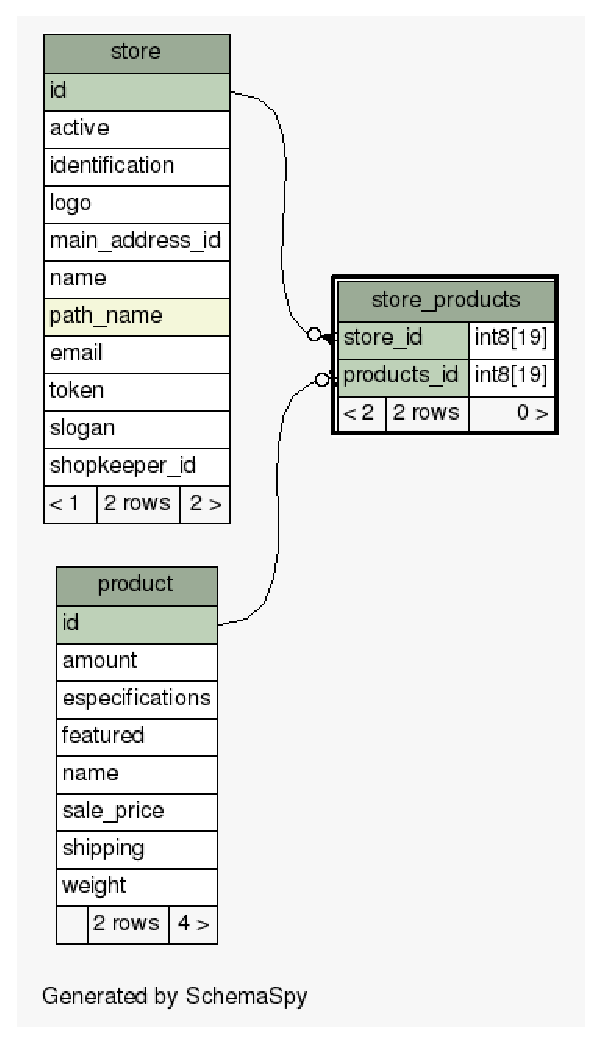
\includegraphics[scale=0.7]{img/diagramas/schema/store_products.1degree.png.eps}\\
\end{figure}

\begin{figure}[H]
\centering
\caption{Pedido e seus relacionamentos}
\centering
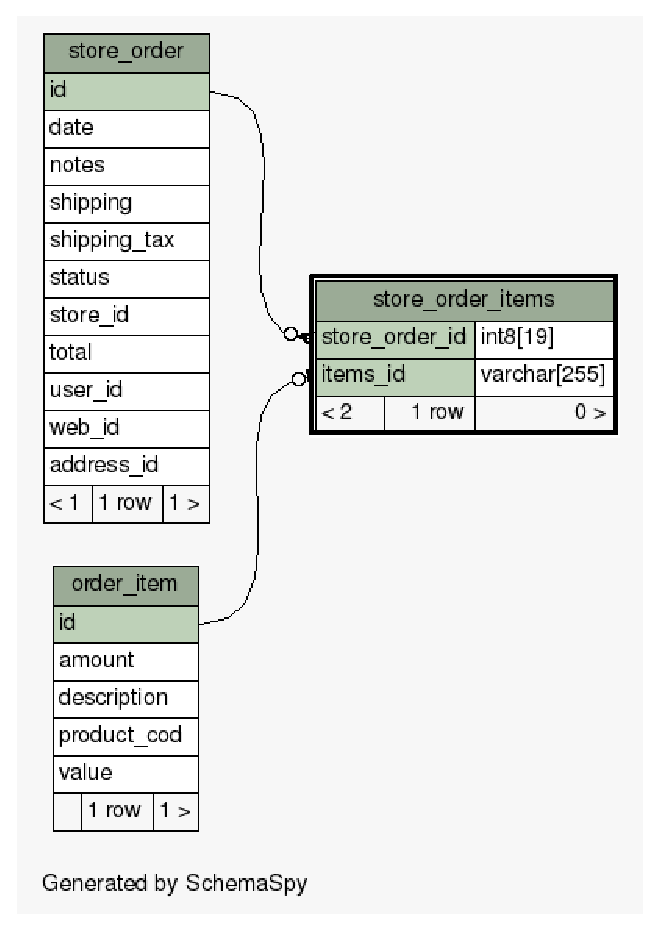
\includegraphics[scale=0.7]{img/diagramas/schema/store_order_items.1degree.png.eps}\\
\end{figure}

\begin{figure}[H]
\centering
\caption{Pedido e seus relacionamentos}
\centering
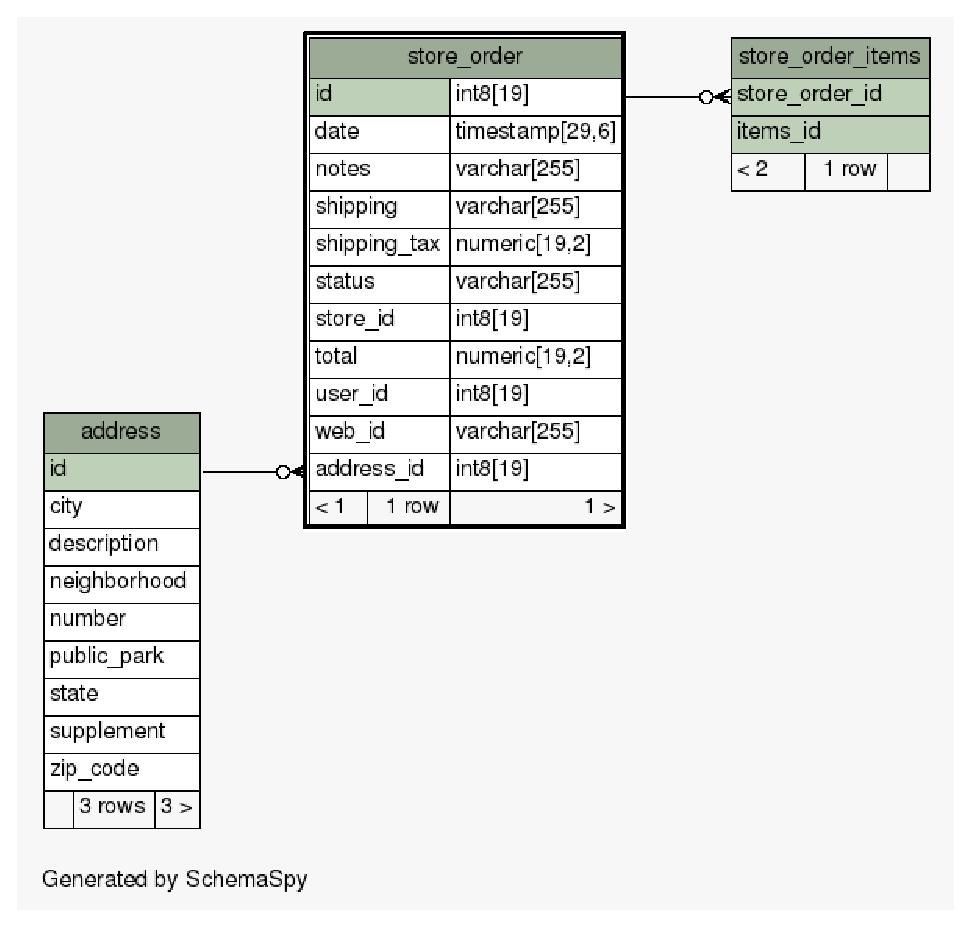
\includegraphics[scale=0.7]{img/diagramas/schema/store_order.1degree.png.eps}\\
\end{figure}

\begin{figure}[H]
\centering
\caption{Endereço e seus relacionamentos}
\centering
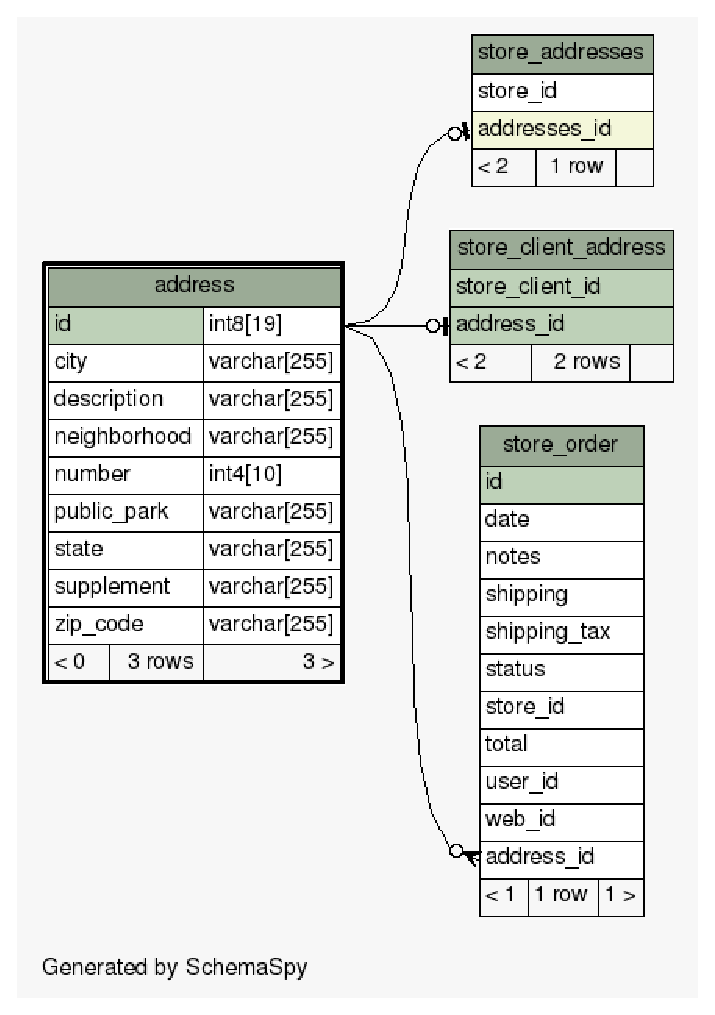
\includegraphics[scale=0.7]{img/diagramas/schema/address.1degree.png.eps}\\
\end{figure}

\begin{figure}[H]
\centering
\caption{Usuário da loja e seus relacionamentos}
\centering
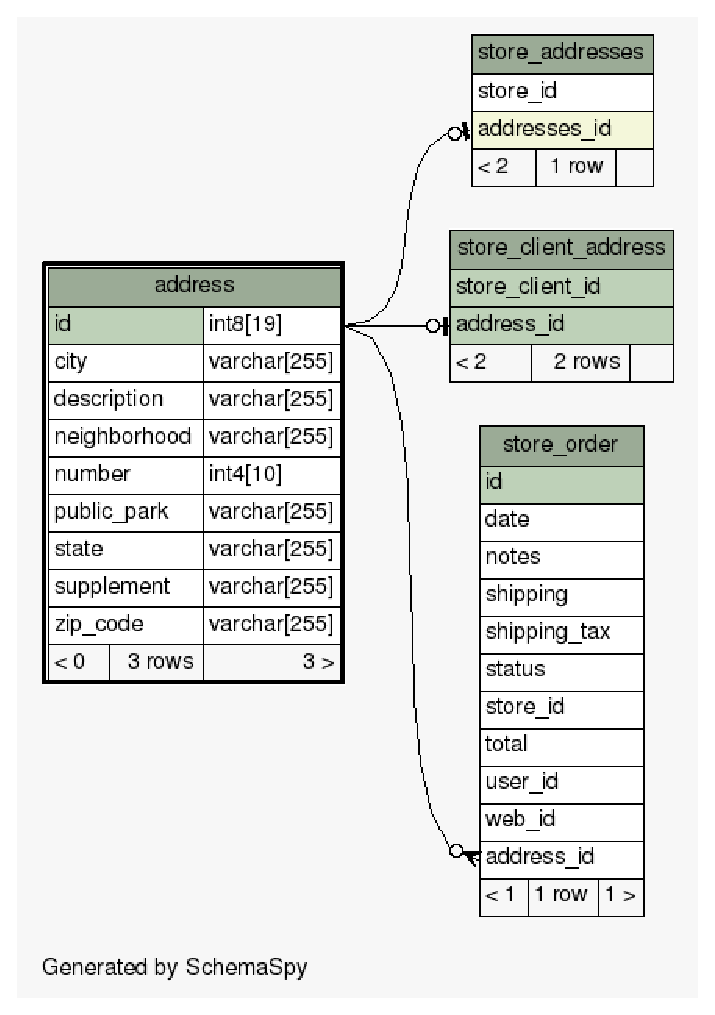
\includegraphics[scale=0.7]{img/diagramas/schema/address.1degree.png.eps}\\
\end{figure}

\begin{figure}[H]
\centering
\caption{Loja e seus relacionamentos}
\centering
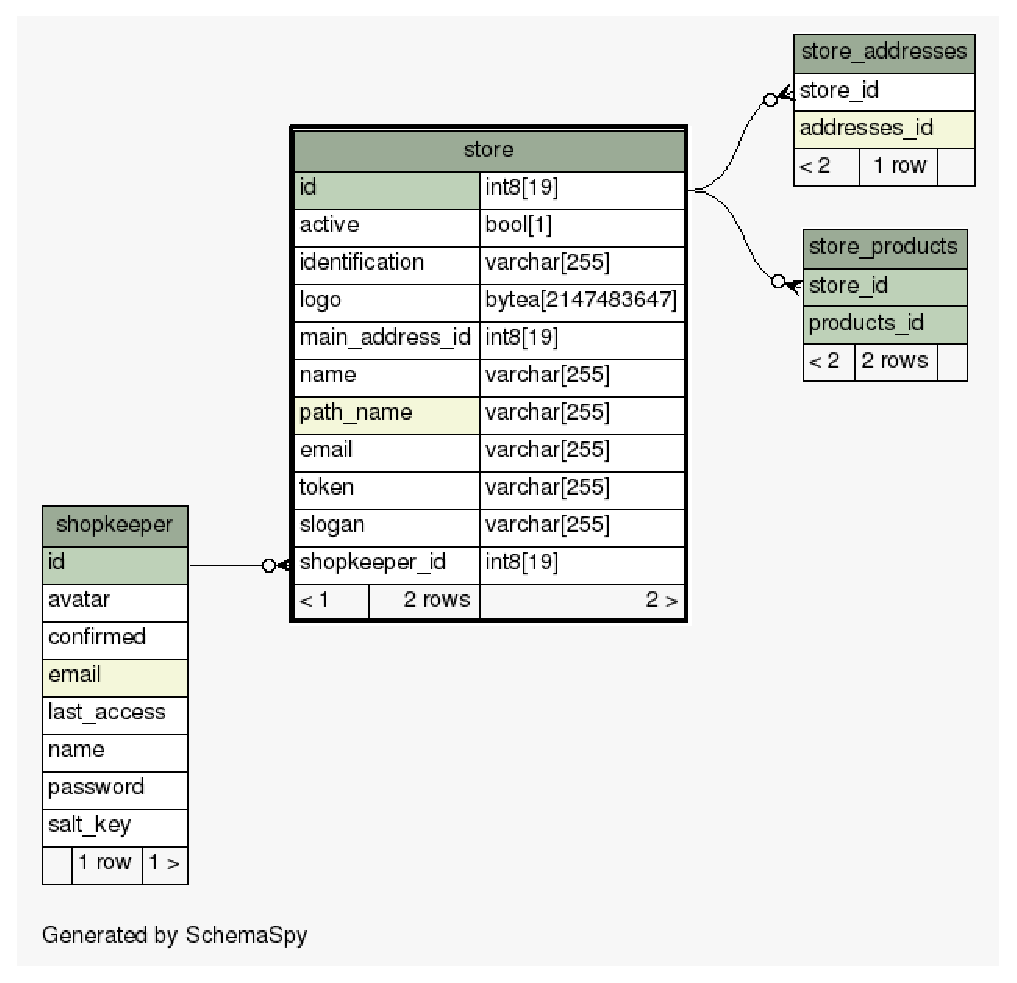
\includegraphics[scale=0.7]{img/diagramas/schema/store.1degree.png.eps}\\
\end{figure}

\begin{figure}[H]
\centering
\caption{Lojista e seus relacionamentos}
\centering
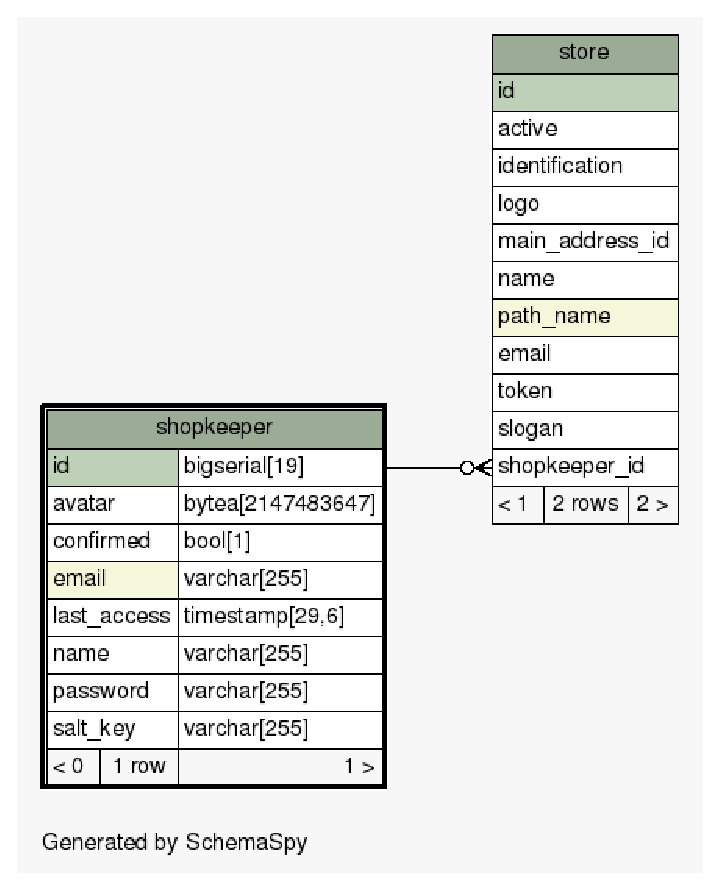
\includegraphics[scale=0.7]{img/diagramas/schema/shopkeeper.1degree.png.eps}\\
\end{figure}

\begin{figure}[H]
\centering
\caption{Produto e seus relacionamentos}
\centering
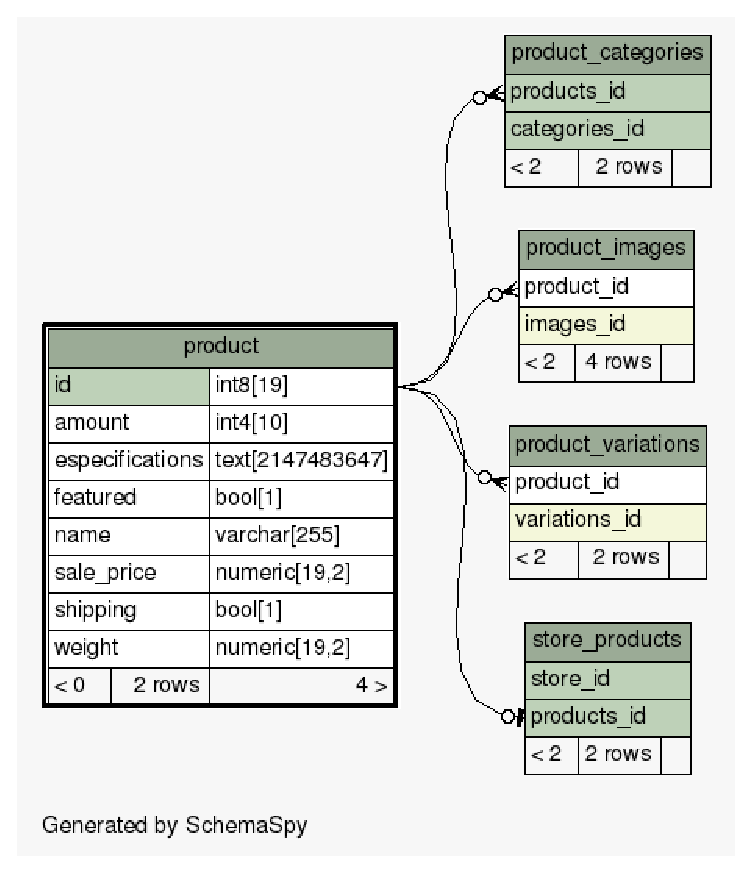
\includegraphics[scale=0.7]{img/diagramas/schema/product.1degree.png.eps}\\
\end{figure}

\begin{figure}[H]
\centering
\caption{Categoria de Produto e seus relacionamentos}
\centering
\includegraphics[scale=0.7]{img/diagramas/schema/product_categories.1degree.png.eps}\\
\end{figure}

\begin{figure}[H]
\centering
\caption{Variação de produto e seus relacionamentos}
\centering
\includegraphics[scale=0.7]{img/diagramas/schema/product_variation.1degree.png.eps}\\
\end{figure}

\begin{figure}[H]
\centering
\caption{Comentários e seus relacionamentos}
\centering
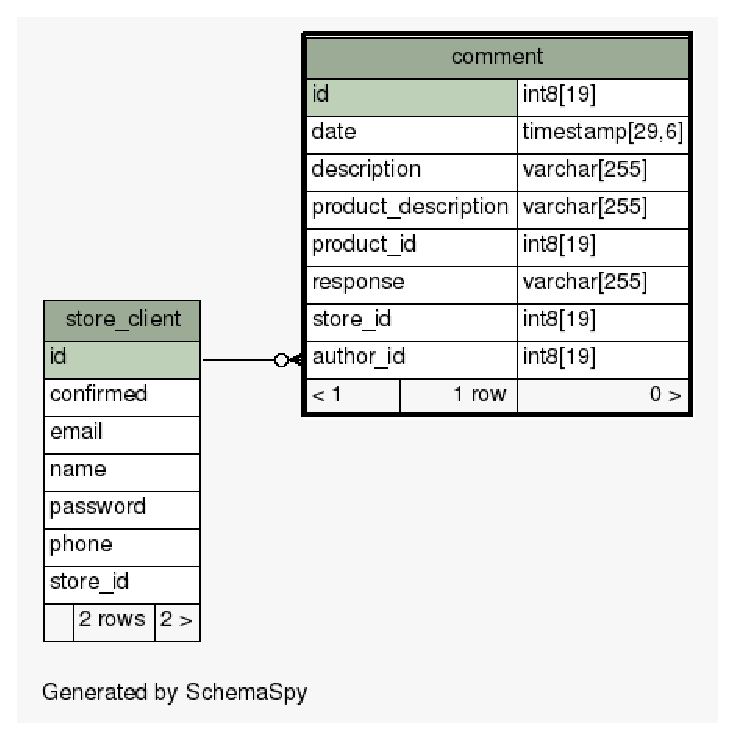
\includegraphics[scale=0.7]{img/diagramas/schema/comment.1degree.png.eps}\\
\end{figure}
% chapter modelo_l_gigo_de_dados (end)

\end{document}
